\documentclass[12pt, usenames, dvipsnames, x11names]{article}
\usepackage[english]{babel}

\usepackage[usenames, dvipsnames, x11names]{xcolor}

\usepackage[letterpaper,top=2cm,bottom=2cm,left=3cm,right=3cm,marginparwidth=1.75cm]{geometry}

\usepackage{amsmath, amsfonts, amsthm, amssymb, gensymb}
\usepackage{graphicx}
\usepackage{svg}

\PassOptionsToPackage{hyphens}{url}\usepackage[hidelinks]{hyperref}

\usepackage{mathptmx}  % Times New Roman
% \usepackage{bookman}  % Bookman
% \usepackage{fourier}  % Fourier
% \usepackage{tgpagella}  % TeX Gyre Pagella


\usepackage{fancyvrb}



\usepackage[skip=10pt plus1pt, indent=0pt]{parskip}

\usepackage[]{mdframed}  % For boxed text

\usepackage[thinlines, thicklines]{easytable}

\usepackage{float}

\usepackage{makecell}

\usepackage{tikz, pgfplots}
\pgfplotsset{compat=1.18}
\usetikzlibrary{arrows.meta, calligraphy}
\usetikzlibrary{calc}

\usepackage{ifthen}

\usepackage{enumitem}

% ------------------------------------------------------

\title{\textbf{COMP0147: Discrete Mathematics for Computer Scientists}}
\author{Raphael Li}
\date{\textit{Year 1 (2024--25), Term 1}}

% ------------------------------------------------------

\newcommand{\setvert}{\;\vert\;}

\newcommand{\TruthTableTrue}{\textbf{\color{ForestGreen} TRUE}}
\newcommand{\TruthTableFalse}{\textbf{\color{BrickRed} FALSE}}

\newcommand{\termnotationdef}[3]{
\textbf{#1}

#2

\textit{#3}
}

\newcommand{\termdesc}[2]{
\textbf{#1}

#2
}

\newcommand{\abs}[1]{\vert #1 \vert}

\DeclareMathOperator{\sgn}{sgn}

% ------------------------------------------------------

\begin{document}
\maketitle

% \begin{mdframed}[linewidth=1pt]
% \noindent This is a first-year course for Computer Science, introducing students to material they will need in future computer science courses and providing basic tools for problem solving.
% \end{mdframed}

\newpage
\tableofcontents

\newpage
\section{Introduction to mathematical reasoning}

Many mathematical properties can be formulated in plain English, but may look ambiguous or unclear to the uninitiated. It is thus essential for us to formulate them in the precise language of logic instead. Before we dive into this methodical approach though, we must first introduce the notion of a set.


\subsection{What is a set?}

A \textit{set} is a collection of different things. It can be thought of as a bag containing a number of different objects. Each object is called an \textit{element} of the set. A set \(S\) containing elements \(a\), \(b\) and \(c\) is denoted as \(S = \{a, b, c\}\). A set has no structure and no order, meaning that \(\{a, b, c\} = \{c, a, b\} = \{c, b, a\}\).

If \(d\) is an element of \(S\), we can denote this by \(d \in S\).

Also, note that:
%
\begin{itemize}
    \item \(\mathbb{N}\) refers to the set of natural numbers. \[0, 1, 2, 3, \cdots\]
    \item \(\mathbb{Z}\) refers to the set of integers: \[\cdots -3, -2, -1, 0, 1, 2, 3, \cdots\]
    \item \(\mathbb{R}\) refers to the set of real numbers.
\end{itemize}


\subsection{Conjunction, disjunction and negation}

Now that we know what is a set is, let us look at a few operators commonly used in mathematical logic:

\begin{itemize}
    \item The binary connective AND represents a \textit{conjunction} and is denoted with the symbol \(\land\). The statement \(P \land Q\) is true when both \(P\) and \(Q\) are true.
    \item The binary connective OR represents a \textit{disjunction} and is denoted with the symbol \(\lor\). The statement \(P \lor Q\) is true when at least one of \(P\) and \(Q\) are true.
    \item The unary connective NOT represents a \textit{negation} and is denoted with the symbol \(\neg\). The statement \(\neg P\) is true when \(P\) is false.
\end{itemize}

The truth tables for \(P\land Q\) and \(P \lor Q\) are shown in tables \ref{tab:Ch1-truth-table-and} and \ref{tab:Ch1-truth-table-or} respectively.

\begin{table}[H]
    \centering
    \begin{tabular}{|c|c|c|}
        \hline
        & \(P\) is true & \(P\) is false \\
        \hline
        \(Q\) is true & \TruthTableTrue & \TruthTableFalse\\
        \hline
        \(Q\) is false & \TruthTableFalse & \TruthTableFalse\\
        \hline
    \end{tabular}
    \caption{The truth table for \(P\land Q\).}
    \label{tab:Ch1-truth-table-and}
\end{table}

\begin{table}[H]
    \centering
    \begin{tabular}{|c|c|c|}
        \hline
        & \(P\) is true & \(P\) is false \\
        \hline
        \(Q\) is true & \TruthTableTrue & \TruthTableTrue\\
        \hline
        \(Q\) is false & \TruthTableTrue & \TruthTableFalse\\
        \hline
    \end{tabular}
    \caption{The truth table for \(P \lor Q\). Note that OR is \textit{not} exclusive here.}
    \label{tab:Ch1-truth-table-or}
\end{table}


\subsection{De Morgan's Laws: Negating conjunctions and disjunctions}

To negate a conjunction or disjunction, we have to ask ourselves: ``In what cases is that conjunction or disjunction false?''

This gives us the following set of relationships, known as De Morgan's Laws or as the Duality Principle.
%
\begin{align*}
    \neg (A \land B) &= \neg A \lor \neg B\\
    \neg (A \lor B) &= \neg A \land \neg B
\end{align*}

For example, consider the following statements:
%
\begin{itemize}
    \item The weather is cold and rainy.
    \item \(f(x) = 0\) or \(g(x) = 0\).
\end{itemize}
%
Their respective negations are as follows:
%
\begin{itemize}
    \item The weather is not cold or not rainy.
    \item \(f(x) \neq 0\) and \(g(x) \neq 0\).
\end{itemize}


\subsection{Implications and their negations}

The binary connective IF... THEN represents an \textit{implication} and is denoted with the symbol \(\Rightarrow\). If \(P \Rightarrow Q\), we can describe this relationship in plain English as:
\begin{itemize}
    \item \(P\) implies \(Q\).
    \item Whenever \(P\) is true, \(Q\) must be true.
    \item \(P\) is a sufficient condition for \(Q\).
    \item \(Q\) is a necessary condition for \(P\).
\end{itemize}

Given an implication \(P \Rightarrow Q\), its \textit{converse} is defined as the statement \(Q \Rightarrow P\). An implication is not always equivalent to its converse.

If we look at the truth table of this connective (table \ref{tab:Ch1-truth-table-if-then}), we may notice that the implication is much more subtle than it might seem at first glance.

\begin{table}[H]
    \centering
    \begin{tabular}{|c|c|c|}
        \hline
        & \(P\) is true & \(P\) is false \\
        \hline
        \(Q\) is true & \TruthTableTrue & \TruthTableTrue\\
        \hline
        \(Q\) is false & \TruthTableFalse & \TruthTableTrue\\
        \hline
    \end{tabular}
    \caption{The truth table for \(P \Rightarrow Q\).}
    \label{tab:Ch1-truth-table-if-then}
\end{table}

The first column is relatively straightforward --- when \(P\) is true, \(Q\) must be true too. The second column, however, is not as intuitive: when \(P\) is false, \(Q\) can be either true or false. This is because the implication \(P \Rightarrow Q\) makes no claims about when \(P\) is false. (This subtlety is often the source of many misunderstandings; for more, see the \href{https://en.wikipedia.org/wiki/Wason_selection_task}{Wikipedia article on the Wason selection task}.)

It might be useful to remember that an implication is false in one scenario only (when \(P\) is true and \(Q\) is false).

Further examination of the truth table reveals that the implication \(P \Rightarrow Q\) can in fact be rewritten as a disjunction:
%
\[P \Rightarrow Q = \neg P \lor Q\]
%
This allows us to easily negate implications:
%
\[\neg (P \Rightarrow Q) = P \land \neg Q\]
%
We can verify this negation by checking its truth table.

\begin{table}[H]
    \centering
    \begin{tabular}{|c|c|c|}
        \hline
        & \(P\) is true & \(P\) is false \\
        \hline
        \(Q\) is true & \TruthTableFalse & \TruthTableFalse\\
        \hline
        \(Q\) is false & \TruthTableTrue & \TruthTableFalse\\
        \hline
    \end{tabular}
    \caption{The truth table for \(\neg (P \Rightarrow Q) = P \land \neg Q\).}
    \label{tab:Ch1-truth-table-negated-implication}
\end{table}

As an example, the statement ``if \(n\) is even, then \(P(n) = 0\)'' can be negated into ``\(n\) is even and \(P(n) \neq 0\)''.



\subsection{Contraposition}

By rewriting an implication as a disjunction, we can show that \(P \Rightarrow Q\) is equivalent to \(\neg Q \Rightarrow \neg P\):
%
\begin{align*}
    P \Rightarrow Q &= \neg P \lor Q\\
    &= Q \lor \neg P\\
    &= \neg (\neg Q) \lor \neg P\\
    &= \neg Q \Rightarrow \neg P
\end{align*}
%
Here, \(\neg Q \Rightarrow \neg P\) is known as the \textit{contrapositive} form. Intuitively this makes sense because if we don’t have \(Q\), we cannot have \(P\).


\subsection{Equivalence}

So far we've been using equal signs to denote that two statements are equal. In mathematical logic, this is often replaced by the binary connective \(\Leftrightarrow\), which represents \textit{equivalence}. Two statements \(P\) and \(Q\) are said to be equal when their properties coincide exactly, i.e. \(P\) implies \(Q\) and \(Q\) implies \(P\).

Given an equivalence \(P \Leftrightarrow Q\), we can describe this in plain English as:
\begin{itemize}
    \item \(P\) is equivalent to \(Q\).
    \item \(P\) if and only if \(Q\). (The phrase ``if and only if'' is usually abbreviated to ``iff''.)
\end{itemize}


\subsection{Quantifiers and their negations}

\textit{Quantifiers} are logical connectives that allow us to reason about variables.

One example is the \textit{universal quantifier} ``for all'', which is denoted as \(\forall\). Given a proposition \(P(x)\) involving \(x\), we can write:
%
\begin{itemize}
    \item For all \(x\), \(P(x)\)
    \item \(\forall x, P(x)\)
\end{itemize}
%
We can also specify that \(x\) must be an element of a certain set \(S\):
%
\begin{itemize}
    \item For all \(x\) in \(S\), \(P(x)\)
    \item \(\forall x \in S,\; P(x)\)
    \item \(\forall x,\; x \in S \Rightarrow P(x)\)
\end{itemize}
%
We can write this in mathematical logic as \(P(s_1) \land P(s_2) \land \cdots \land P(s_n)\), where \(s_1, s_2, \cdots, s_n\) are elements of \(S\).

Another example of a quantifier is the \textit{existential quantifier} ``there exists'', denoted as \(\exists\). Given a proposition \(P(x)\) involving \(x\), we can write:
%
\begin{itemize}
    \item There exists \(x\) such that \(P(x)\)
    \item \(\exists x, P(x)\)
\end{itemize}
%
Again we can also specify that \(x\) must be an element of a set \(S\):
%
\begin{itemize}
    \item There exists \(x\) in \(S\) such that \(P(x)\)
    \item \(\exists x \in S,\; P(x)\)
    \item \(\exists x,\; x \in S \land P(x)\)
\end{itemize}
%
This can be written in mathematical logic as \(P(s_1) \lor P(s_2) \lor \cdots \lor P(s_n)\), where \(s_1, s_2, \cdots, s_n\) are elements of \(S\).

To negate a quantifier, we once again ask ourselves the question: In what cases is the quantifier false? This gives the following, which are in fact equivalent to De Morgan's Laws.
%
\begin{itemize}
    \item \(\neg(\forall x, P(x)) = \exists x, \neg P(x)\)
    \item \(\neg(\exists x, P(x)) = \forall x, \neg P(x)\)
\end{itemize}

Lastly, we note the following remarks:
%
\begin{itemize}
    \item It is possible to quantify over several variables. We write \(\forall x, y\) as a shortcut for \(\forall x, \forall y\).

    \item When a statement consists of multiple quantifiers, their order matters. The statement \(\forall x, \exists y, P(x, y)\) is \textit{not} equivalent to \(\exists y, \forall x, P(x, y)\). To illustrate this we can consider the statements \(\forall x \in \mathbb{R}, \exists y \in \mathbb{R}, x < y\) and \(\exists y \in \mathbb{R}, \forall x \in \mathbb{R}, x < y\). These two statements are not equivalent: the former is true but the latter is false.
    
    \item For any statements \(P(x)\) and \(Q(x)\), we have
    %
    \begin{align*}
        \exists x, (P(x) \lor Q(x)) &\Leftrightarrow (\exists x, P(x)) \lor (\exists x, Q(x))\\
        \forall x, (P(x) \land Q(x)) &\Leftrightarrow (\forall x, P(x)) \land (\forall x, Q(x))
    \end{align*}
    %
    However, in general,
    %
    \begin{align*}
        \exists x, (P(x) \land Q(x)) &\not\Leftrightarrow (\exists x, P(x)) \land (\exists x, Q(x))\\
        \forall x, (P(x) \lor Q(x)) &\not\Leftrightarrow (\forall x, P(x)) \lor (\forall x, Q(x))
    \end{align*}

    \item Let \(P\) be a statement that does not involve \(x\) whatsoever. Then:
    %
    \begin{align*}
        \exists x, (P \lor Q(x)) &\Leftrightarrow P \lor \exists x, Q(x)\\
        \exists x, (P \land Q(x)) &\Leftrightarrow P \land \exists x, Q(x)\\
        \forall x, (P \lor Q(x)) &\Leftrightarrow P \lor \forall x, Q(x)\\
        \forall x, (P \land Q(x)) &\Leftrightarrow P \land \forall x, Q(x)\\
        \forall x, (P \Rightarrow Q(x)) &\Leftrightarrow P \Rightarrow \forall x, Q(x)\\
        \forall x, (Q(x) \Rightarrow P) &\Leftrightarrow (\exists x, Q(x)) \Rightarrow P
    \end{align*}
\end{itemize}


\subsection{Proving and disproving mathematical propositions}

\begin{itemize}
    \item To prove \(P \land Q\), we must prove both \(P\) and \(Q\). To disprove it, we must prove \(\neg (P \land Q) = \neg P \lor \neg Q\) (by De Morgan's Laws).
    
    \item To prove \(P \lor Q\), we must prove \(P\) or \(Q\), even though we might not necessarily know which one is true. To disprove it, we must prove \(\neg (P \lor Q) = \neg P \land \neg Q\) (by De Morgan's Laws).
    
    \item To prove \(P \Rightarrow Q\), we begin by assuming \(P\) is true and then show that \(Q\) is also true. To disprove it, we must find a \textit{counterexample} where \(P\) is true but \(Q\) is false.
    
    \item To prove \(P \Leftrightarrow Q\), we must prove \(P \Rightarrow Q \land Q \Rightarrow P\). Both implications must be proved. To disprove it, we must prove that either \(P \Rightarrow Q\) is false, or \(Q \Rightarrow P\), or both.
    
    \item To prove \(\forall x \in S, P(x)\), we begin our proof with the line ``let \(x \in S\)'', without specifying the value of \(x\). We then prove the property \(P(x)\). To disprove it, we must find a counterexample where \(x\) is an element of \(S\) but does not satisfy the property \(P(x)\).

    \item To prove \(\exists x \in S, P(x)\), we must find an example of \(x\) where \(x\) is an element of \(S\) and satisifies the property \(P(x)\). To disprove it, we must show that for all \(x \in S\), the statement \(P(x)\) is false.
\end{itemize}



\subsection{Free and bound variables}

Variables can be more complicated than they appear to be. Consider the following statement.
%
\[P({\color{MidnightBlue} x }) = (Q({\color{MidnightBlue} x }) \Rightarrow \forall {\color{BrickRed} x }, Q({\color{BrickRed} x }))\]
%
Note that the blue instances of \(x\) can be replaced by any value (e.g. 4, 6.1, etc.) and the statement would still be understandable. These are known as \textit{free} variables. On the contrary, the red instances are ``untouchable'' and cannot be replaced; they can only be renamed. They are known as \textit{bound} variables.

Once you understand the different between free and bound variables, you'll notice them everywhere:
\begin{itemize}
    \item In summation:
    \[\sum_{{\color{BrickRed}i}=1}^{{\color{MidnightBlue}n}} {\color{BrickRed}i}^2\]

    \item In integral calculus:
    \[\int_{a}^{\color{MidnightBlue}b} \sin{(2 {\color{BrickRed} t} +1)}\; d {\color{BrickRed} t}\]

    \item In programming, specifically the use of local and global variables.
\end{itemize}



\newpage
\section{Set theory}

In the previous section, we defined a set as a collection of elements. In this section, we will examine how sets interact with each other, and how their interactions are governed by various laws and properties.


\subsection{Basic set notation}

We can define a set using set-builder notation. For example, if we want to define \(A\) as the set of all real numbers \(x\) where \(x^2 = x\), we can use any of the two definitions shown below:
%
\begin{align*}
    A &= \{x \setvert x \text{ is a real number s.t. } x^2 = x\}\\
    A &= \{x : x^2 = x\}
\end{align*}

Consider the sets \(X = \{2, 4\}\) and \(Y = \{1, 2, 3, 4, 5\}\). Notice that for every element in \(X\), that element also appears in \(Y\), i.e.
%
\[\forall x,\; x \in X \implies x \in Y\text{.}\]
%
When this happens, we say that \(X\) is a subset of \(Y\), denoted as \(X \subseteq Y\).

The \textit{cardinality} of a set \(S\) refers to the number of elements in it, and is denoted as \(\abs{S}\). A set that contains no elements is known as an \textit{empty set} and is denoted as \(\emptyset\). Contrarily, a set that contains all possible elements is known as the \textit{universal set} and is denoted as \(U\).

For any set \(S\), the power set \(P(S)\) is the set of all subsets of \(S\). If \(S\) has \(n\) elements, then \(P(S)\) will have \(2^n\) elements. For example, if \(S = \{0, 1\}\), then \(P(S) = \{\emptyset, \{0\}, \{1\}, \{0, 1\}\}\).


\subsection{Set operations}

We introduce the following set operations.

\begin{enumerate}\setlength\itemsep{1.5em}
    \item\termnotationdef{Union}{\(A \cup B = \{x \setvert (x \in A) \lor (x \in B)\}\)}{The union of two sets \(A\) and \(B\) refers to the set of all elements that are found in either \(A\) or \(B\).}

    \item\termnotationdef{Intersection}{\(A \cap B = \{x \setvert (x \in A) \land (x \in B)\}\)}{The intersection of two sets \(A\) and \(B\) refers to the set of all elements that are found in both \(A\) and \(B\).}

    \item\termnotationdef{Difference}{\(A \backslash B = \{x \setvert (x \in A) \land (x \notin B)\}\)}{The difference between two sets \(A\) and \(B\), or ``\(A\) minus \(B\)'', refers to the set of all elements that are found in \(A\) but not \(B\). Note that \(A \backslash B\) is different from \(B \backslash A\).}

    \item\termnotationdef{Symmetric difference}{\(A \Delta B = (A \backslash B) \cup (B \backslash A) = (A \cup B) \backslash (A \cap B)\)}{The symmetric difference between two sets \(A\) and \(B\) refers to the set of all elements that are found in either \(A\) or \(B\), but not both.}

     \item\termnotationdef{Complement}{\(A^c = U \backslash A\)}{The complement of a set \(A\) refers to the set of all elements that are not found in \(A\).}

     \item\termnotationdef{Cartesian product}{\(A \times B = \{(a, b) \setvert (a \in A) \land (b \in B)\}\)}{The Cartesian product of two sets \(A\) and \(B\) refers to the set of all ordered pairs \((a, b)\) where \(a\) is an element of \(A\) and \(b\) is an element of \(B\).}
\end{enumerate}

\begin{figure}[h]
    \centering
    \includegraphics[width=0.95\linewidth]{Images/Ch2/SetNotation.jpg}
    \caption{From left to right, top to bottom: Venn diagram representations of \(A\cup B\), \(A \cap B\), \(A \backslash B\), \(A \Delta B\) and \(A^c\), along with a representation of the Cartesian product \(A \times B\) using the Cartesian coordinate system.}
    \label{fig:Ch2-set-notation-visualization}
\end{figure}

When expressing the union or intersection of a large number of sets, we can use the following shorthand:
%
\begin{align*}
    \bigcup\limits_{m \in M} A_m &= A_{m_1} \cup A_{m_2} \cup A_{m_3} \cup \cdots \cup A_{m_n}\\
    \bigcap\limits_{m \in M} A_m &= A_{m_1} \cap A_{m_2} \cap A_{m_3} \cap \cdots \cap A_{m_n}
\end{align*}
%
where \(M = \{m_1, m_2, m_3, \cdots m_n\}\).





\subsection{Set algebra}

\subsubsection{Similarities between sets, logic and arithmetic}

Set algebra concerns properties of sets and set operations. Before we delve into these properties though, let us first acknowledge the following fact:
%
\begin{quote}
    The way the set operations \(A \cup B\) and \(A \cap B\) behave is very similar to that of the logical operations \(A \lor B\) and \(A \land B\), and also that of the arithmetic operations \(A+B\) and \(A\cdot B\).
\end{quote}

This is expressed more concisely with in table \ref{tab:Ch2-mirroring-behavior-set-logical-arithmetic}. 

\begin{table}[h]
    \centering
    \begin{tabular}{|c||c|c|}
        \hline
        \textbf{Set operations} & \(A \cup B\) & \(A \cap B\)\\
        \hline
        \textbf{Logical operations} & \(A \lor B\) & \(A \land B\)\\
        \hline
        \textbf{Arithmetic operations} & \(A+B\) & \(A\cdot B\)\\
        \hline
    \end{tabular}
    \caption{The behaviours of these operations mirror one another almost identically.}
    \label{tab:Ch2-mirroring-behavior-set-logical-arithmetic}
\end{table}

To illustrate this fact, table \ref{tab:Ch2-laws-set-logical-arithmetic} introduces a number of laws in set algebra and compares them to their counterparts in mathematical logic and arithmetic. For each of the four laws, note the structural similarities in regard to how the law is applied in sets, in logic and in arithmetic.

\begin{table}[H]
    \scriptsize
    \centering
    \begin{tabular}{|p{0.1\textwidth}|p{0.25\textwidth}|p{0.25\textwidth}|p{0.25\textwidth}|}
       
        \hline
        
        & \makecell{\textbf{In sets}\\ (\(\cup,\; \cap\))}
        & \makecell{\textbf{In logic}\\ (\(\lor,\; \land\))}
        & \makecell{\textbf{In arithmetic}\\ (\(+,\; \cdot\))}
        \\
        
        \hline
        
        \textbf{Commutative}
        & {\makecell{\(\begin{aligned}
            A \cup B &= B \cup A\\
            A \cap B &= B \cap A
        \end{aligned}\)}}
        & {\makecell{\(\begin{aligned}
            A \lor B &= B \lor A\\
            A \land B &= B \land A
        \end{aligned}\)}}
        & {\makecell{\(\begin{aligned}
            A + B &= B + A\\
            A \cdot B &= B \cdot A
        \end{aligned}\)}}
        \\
        
        \hline
        
        \textbf{Associative}
        & {\makecell{\(\begin{aligned}
            A \cup (B \cup C) &= (A \cup B) \cup C\\
            A \cap (B \cap C) &= (A \cap B) \cap C\\
        \end{aligned}\)}}
        & {\makecell{\(\begin{aligned}
            A \lor (B \lor C) &= (A \lor B) \lor C\\
            A \land (B \land C) &= (A \land B) \land C\\
        \end{aligned}\)}}
        & {\makecell{\(\begin{aligned}
            A + (B + C) &= (A + B) + C\\
            A \cdot (B \cdot C) &= (A \cdot B) \cdot C
        \end{aligned}\)}}
        \\

        \hline

        \textbf{Distributive}
        & {\makecell{\(\begin{aligned}
            A \cap (B \cup C) &= (A \cap B) \cup (A \cap C)\\
            A \cup (B \cap C) &= (A \cup B) \cap (A \cup C)\\
        \end{aligned}\)}}
        & {\makecell{\(\begin{aligned}
            A \land (B \lor C) &= (A \land B) \lor (A \land C)\\
            A \lor (B \land C) &= (A \lor B) \land (A \lor C)\\
        \end{aligned}\)}}
        & {\makecell{\(\begin{aligned}
            A \cdot (B + C) &= A \cdot B + A \cdot C \\
            &\text{N/A}
        \end{aligned}\)}}
        \\

        \hline

        \textbf{Identity}
        & {\makecell{\(\begin{aligned}
            A \cup \emptyset &= A\\
            A \cap \emptyset &= \emptyset\\
            A \cup U &= U\\
            A \cap U &= A
        \end{aligned}\)}}
        & {\makecell{N/A}}
        & {\makecell{\(\begin{aligned}
            A + 0 &= A\\
            A \cdot 0 &= 0\\
            &\text{N/A}\\
            A \cdot 1 &= 1
        \end{aligned}\)}}
        \\

        \hline

        \textbf{Double complement}
        & {\makecell{\((A^c)^c = A\)}}
        & {\makecell{\(\neg(\neg A) = A\)}}
        & {\makecell{N/A}}
        \\

        \hline

        \textbf{De Morgan's}
        & {\makecell{\(\begin{aligned}
            (A \cup B)^c &= A^c \cap B^c\\
            (A \cap B)^c &= A^c \cup B^c
        \end{aligned}\)}}
        & {\makecell{\(\begin{aligned}
            \neg(A \lor B) &= \neg A \land \neg B\\
            \neg(A \land B) &= \neg A \lor \neg B
        \end{aligned}\)}}
        & {\makecell{N/A}}
        \\

        \hline

        \textbf{Absorption}
        & {\makecell{\(\begin{aligned}
        A \cup (A \cap B) &= A\\
        A \cap (A \cup B) &= A
    \end{aligned}\)}}
        & {\makecell{\(\begin{aligned}
        A \lor (A \land B) &= A\\
        A \land (A \lor B) &= A
    \end{aligned}\)}}
        & {\makecell{N/A}}
        \\

        \hline
        
    \end{tabular}
    \caption{Applying commutative, associative, distributive, identity, double complement, De Morgan's and absorption laws to set algebra, mathematical logic and basic arithmetic.}
    \label{tab:Ch2-laws-set-logical-arithmetic}
\end{table}


\subsubsection{Other miscellaneous laws}

Apart from the laws listed above, we will also introduce a few miscellaneous laws in set algebra.

\begin{enumerate}\setlength\itemsep{1.5em}
    \item \termdesc{Idempotent Laws\footnote{The word ``idempotent'' comes from the Latin root ``idem'' meaning ``same'' and the word ``potent'' which means ``having great power''. As a whole, the word literally translates to ``having the same effect''.}}{\(\begin{aligned}
        A \cup A &= A\\
        A \cap A &= A
    \end{aligned}\)}

    \item \termdesc{General De Morgan's Laws\footnote{This is equivalent to the De Morgan's Laws introduced in table \ref{tab:Ch2-laws-set-logical-arithmetic}, which can be obtained by setting \(C\) to the universal set \(U\).}}{\(\begin{aligned}
        C \backslash (A \cup B) &= (C \backslash A) \cap (C \backslash B)\\
        C \backslash (A \cap B) &= (C \backslash A) \cup (C \backslash B)
    \end{aligned}\)}

    \item \termdesc{De Morgan's Laws for an Arbitrary Number of Sets}{\(\begin{aligned}
        \left(\bigcup\limits_{n \in N} A_n \right)^c &= \bigcap\limits_{n \in N} A^c_n\\
        \left(\bigcap\limits_{n \in N} A_n \right)^c &= \bigcup\limits_{n \in N} A^c_n
    \end{aligned}\)}

    \item \termdesc{Alternative definition of difference}{\(A \backslash B = A \cap B^c\)}

    \item \termdesc{Contraposition}{\(\begin{aligned}
        (A \subseteq B) &\text{ iff } (B^c \subseteq A^c)\\
        (A = B) &\text{ iff } (A^c = B^c)
    \end{aligned}\)}
\end{enumerate}


\subsection{Proving two sets are equivalent}

Consider the two sets defined below.
%
\begin{align*}
    A &= \{x : x^2 = x\}\\
    B &= \{1, 0\}
\end{align*}
%
Intuitively, these two sets should be equivalent, as they contain the same two elements. However, to mathematically prove the equivalence between the sets, we must be able to demonstrate that:
%
\begin{enumerate}
    \item \(A\) is a subset of \(B\), i.e. \(A \subseteq B\); and
    \item \(B\) is a subset of \(A\), i.e. \(B \subseteq A\).
\end{enumerate}
%
These statements must each be proven individually, as shown below.
%
\begin{align*}
    x &\in A \implies x^2 = x \implies (x = 0) \lor (x = 1) \implies x \in B \tag{proof for statement 1}\\
    y &\in B \implies (x = 0) \lor (x = 1) \implies y^2 = y \implies y \in A\tag{proof for statement 2}
\end{align*}


\subsection{Constructing proofs with top-down and bottom-up approach}

In general, proofs in set algebra can be constructed using the ``top-down then bottom-up'' approach:
%
\begin{enumerate}
    \item \textbf{Top-down:} Starting from one side of the equation, reduce that side to the primitive facts.
    \item \textbf{Bottom-up:} Afterwards, combine those primitive facts to reach the other side of the equation.
\end{enumerate}

\vspace{2em}

\begin{mdframed}[linewidth=1pt]
\noindent \textbf{Example}

Prove that \(A \backslash B = A \backslash (A \cap B)\).

\begin{proof}
    We break the equation down into two separate statements. The first statement is equivalent to \(\text{LHS} \subseteq \text{RHS}\) while the second one is equivalent to \(\text{RHS} \subseteq \text{LHS}\).

    \begin{enumerate}
        \item \(\forall x,\; (x \in \text{LHS}) \implies (x \in \text{RHS})\)
        \item \(\forall y,\; (y \in \text{RHS}) \implies (y \in \text{LHS})\)
    \end{enumerate}

    To prove the first statement, note that if \(x \in \text{LHS} = A \backslash B\), then \(x \in A \land x \notin B\) \textit{(top-down)}. Since \(x \notin B\), we have \(x \notin A \cap B\). Recalling that \(x \in A\), we conclude that \(x \in A \backslash (A \cap B) = \text{RHS}\) \textit{(bottom-up)}.

    To prove the second statement, not that if \(y \in \text{RHS} = A \backslash (A \cap B)\), then \(y \in A \land y \notin A \cap B\). This means that \(y \notin B\) \textit{(top-down)}. Since \(y \in A \land y \notin B\), we have \(y \in A\backslash B\) \textit{(bottom-up)}, concluding the proof.
\end{proof}

\end{mdframed}







\newpage
\section{Functions}

\subsection{What is a function?}

\begin{figure}[H]
    \centering
    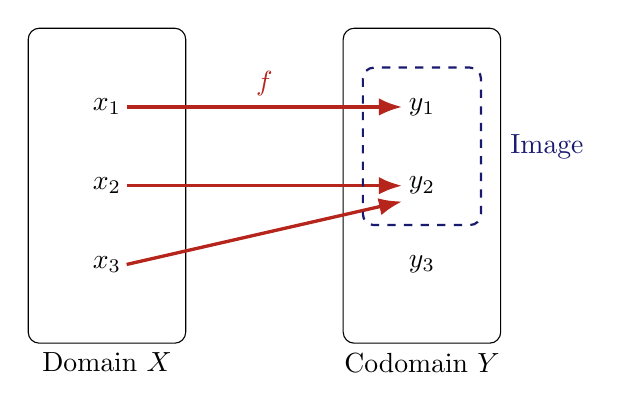
\begin{tikzpicture}
        \draw[rounded corners] (-3, 0) rectangle (-1, -4) {};
        \draw[rounded corners] (1, 0) rectangle (3, -4) {};

        \foreach \i  in {1,...,3} {
            \node[align=center, anchor=center] at (-2, -\i) {\(x_{\i}\)};
        }

        \foreach \i  in {1,...,3} {
            \node[align=center, anchor=center] at (2, -\i) {\(y_{\i}\)};
        }

        \draw[-Latex, very thick, BrickRed] (-1.75, -1) -- (1.75, -1) node[pos=0.5, anchor=south] {\(f\)};

        \draw[-Latex, very thick, BrickRed] (-1.75, -2) -- (1.75, -2);

        \draw[-Latex, very thick, BrickRed] (-1.75, -3) -- (1.75, -2.2);

        \node[anchor=north] at (-2, -4) {Domain \(X\)};

        \node[anchor=north] at (2, -4) {Codomain \(Y\)};

        \draw[rounded corners, MidnightBlue, dashed, thick] (1.25, -0.5) rectangle (2.75, -2.5) {};

        \node[anchor=west, MidnightBlue, align=left] at (3, -1.5) {Image};
        
    \end{tikzpicture}
    \caption{A function, its domain, its codomain and its image.}
    \label{fig:Ch3-function}
\end{figure}

Let \(X\) and \(Y\) be sets. Suppose we have a rule \(f\) that assigns (or ``maps'') each element \(x \in X\) to a unique element \(y \in Y\). This is called a \textit{function} or \textit{mapping}, and is notated as \(y = f(x)\) and \(f : X \rightarrow Y\). The set \(X\) is known as the \textit{domain} of \(f\) while \(Y\) is the \textit{codomain} of \(f\). This is illustrated in figure \ref{fig:Ch3-function}.

We also define the \textit{image} of \(f\) as \(\{y \in Y : \exists x \in X, f(x) = y\}\). Plainly put, the image of a function is the set of all its possible outputs. This is shown in blue in the above diagram.

Note that it is not necessary for all the elements in the codomain to also be elements of the image. Referring back to the diagram, there is no input in \(X\) that could possibly result in the output \(y_3\). In other words, \(y_3\) is in the codomain of \(f\), but not in its image.


\subsection{Total and partial functions}

Consider the function \(f(x) = \sqrt{x}\). Both its domain and codomain are the set of real numbers, i.e. \(f : \mathbb{R} \rightarrow \mathbb{R}\).

Except not really: The function only accepts non-negative numbers as inputs. This kind of function, where it's only defined on a subset of its domain, is called a \textit{partial function}. The opposite of a partial function is a \textit{total function}, which is defined for all elements in its domain.

\begin{figure}[H]
    \centering
    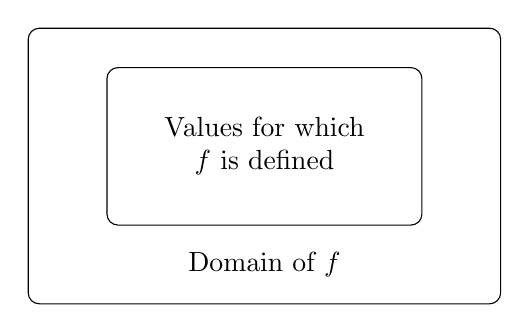
\begin{tikzpicture}
        \draw[rounded corners] (-2,0) rectangle (2,-2);

        \draw[rounded corners] (-3,0.5) rectangle (3,-3);

        \node[align=center] at (0,-1)  {Values for which\\ \(f\) is defined};

        \node[align=center] at (0,-2.5)  {Domain of \(f\)};
    \end{tikzpicture}
    \caption{A partial function \(f\) is only defined for a subset of its domain.}
    \label{fig:ch3-partial-function-maths}
\end{figure}

This distinction between total and partial functions can be generalized to the functions we see in code. For example, consider the following function written in C.
%
\begin{quote}
\begin{verbatim}
int func(int x) {
    do {
        x *= 2;
    } while (!x);
    
    return x;
}
\end{verbatim}
\end{quote}
%
Here, \verb|func| accepts an \verb|int| as input, multiplies it by 2, and returns the product as output. There's just one exception: if we execute the function with input \verb|x = 0|, the function would spiral into an infinite loop without ever producing an output. In other words, the program does not \textit{terminate}.

\begin{table}[H]
    \centering
    \begin{tabular}{|c|c|}
        \hline
        \textbf{Input} & \textbf{Output}\\
        \hline
        -2 & -4 \\
        \hline
        -1 & -2 \\
        \hline
        0 & \textit{(Infinite loop)}\\
        \hline
        1 & 2\\
        \hline
        2 & 4\\
        \hline
    \end{tabular}
    \caption{Examples of inputs and outputs for the \texttt{func} function.}
    \label{tab:ch3-func-input-and-output}
\end{table}

This means that \verb|func| is a partial function: its domain is all values of type \verb|int|, but it only terminates for non-zero inputs.

\begin{figure}[H]
    \centering
    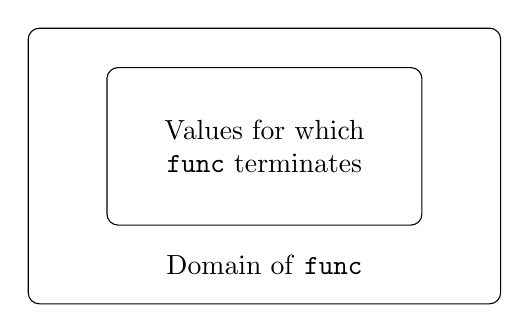
\begin{tikzpicture}
        \draw[rounded corners] (-2,0) rectangle (2,-2);

        \draw[rounded corners] (-3,0.5) rectangle (3,-3);

        \node[align=center] at (0,-1)  {Values for which\\ \texttt{func} terminates};

        \node[align=center] at (0,-2.5)  {Domain of \texttt{func}};
    \end{tikzpicture}
    \caption{A partial function \texttt{func} only terminates for input values from a subset of its domain.}
    \label{fig:ch3-partial-function-cs}
\end{figure}

As a sidenote, it is impossible for an algorithm to take a function as an input and determine whether that function terminates or not. This is known as the \textit{halting problem} (or \textit{entscheidungsproblem}). In 1936, Alan Turing proved that the halting problem is generally undecidable.


\subsection{Seqential composition of functions}

Consider the functions \(f : X \rightarrow Y\) and \(g : Y \rightarrow Z\).

In mathematics, we can create a composition of these two functions \(h(x) = g(f(x))\), where \(h : X \rightarrow Z\). Here, we first apply \(f\) to the input value, and then apply \(g\) to give the output. This is denoted as
%
\[h = g \circ f\text{.}\]
%
Notice how the function that is applied first (\(f\)) is written on the right.

In computer science, we can similarly define the composition of two functions in accordance with the sequential composition paradigm. We use the following notation.
%
\[h = f; g\]
%
where the functions are written in the order in which they are applied. A semicolon is used to separate the composited functions, similar to how we use semicolons to separate consecutive statements in many programming languages.


\subsection{Injections (encodings)}

A function \(f : X \rightarrow Y\) is \textit{injective} if
%
\[\forall a, b \in X,\; f(a) = f(b) \Rightarrow a = b\]
%
or
%
\[\forall a, b \in X,\; a \neq b \Rightarrow f(a) \neq f(b)\text{.}\]
%
These two definitions are contrapositives of each other and are thus equivalent. An injective function is called an \textit{injection} or an \textit{encoding}.

\begin{figure}[H]
    \centering
    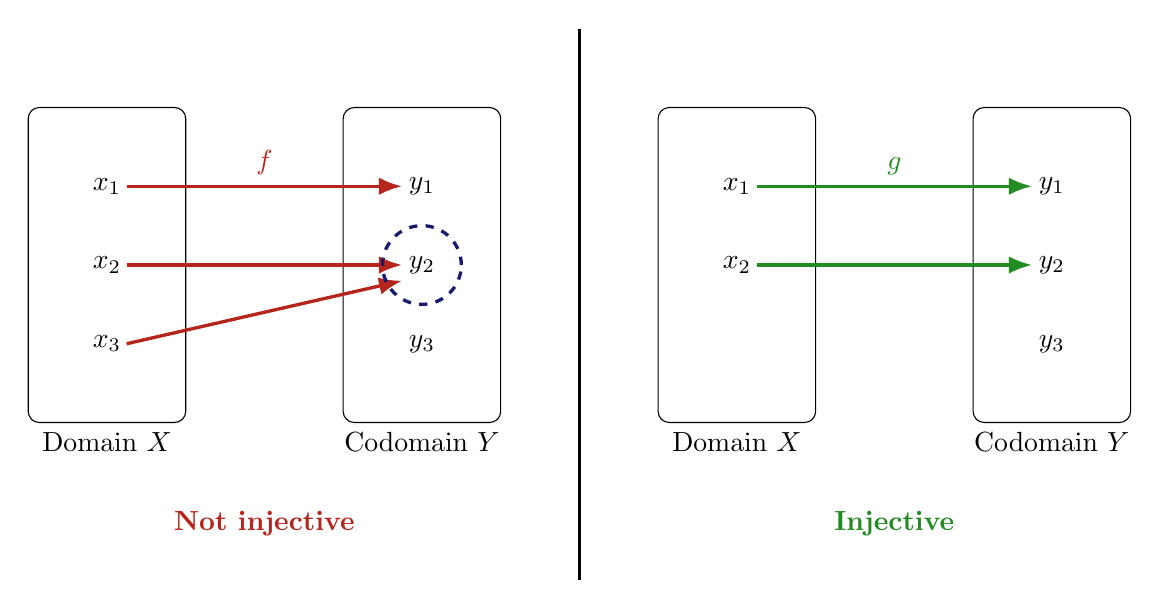
\begin{tikzpicture}
        \draw[rounded corners] (-3, 0) rectangle (-1, -4) {};
        \draw[rounded corners] (1, 0) rectangle (3, -4) {};

        \foreach \i  in {1,...,3} {
            \node[align=center, anchor=center] at (-2, -\i) {\(x_{\i}\)};
        }

        \foreach \i  in {1,...,3} {
            \node[align=center, anchor=center] at (2, -\i) {\(y_{\i}\)};
        }

        \draw[-Latex, very thick, BrickRed] (-1.75, -1) -- (1.75, -1) node[pos=0.5, anchor=south] {\(f\)};

        \node[anchor=north, BrickRed, align=left] at (0, -5) {\textbf{Not injective}};

        \draw[-Latex, very thick, BrickRed] (-1.75, -2) -- (1.75, -2);

        \draw[-Latex, very thick, BrickRed] (-1.75, -3) -- (1.75, -2.2);

        \draw[MidnightBlue, very thick, dashed] (2,-2) circle [radius=0.5];

        \node[anchor=north] at (-2, -4) {Domain \(X\)};

        \node[anchor=north] at (2, -4) {Codomain \(Y\)};

        \draw[thick] (4, 1) -- (4, -6);
        
        \begin{scope}[shift={(8, 0)}]
            \draw[rounded corners] (-3, 0) rectangle (-1, -4) {};
            \draw[rounded corners] (1, 0) rectangle (3, -4) {};
    
            \foreach \i  in {1,2} {
                \node[align=center, anchor=center] at (-2, -\i) {\(x_{\i}\)};
            }
    
            \foreach \i  in {1,...,3} {
                \node[align=center, anchor=center] at (2, -\i) {\(y_{\i}\)};
            }
    
            \draw[-Latex, very thick, ForestGreen] (-1.75, -1) -- (1.75, -1) node[pos=0.5, anchor=south] {\(g\)};

            \node[anchor=north, ForestGreen, align=left] at (0, -5) {\textbf{Injective}};
            
            \draw[-Latex, very thick, ForestGreen] (-1.75, -2) -- (1.75, -2);
    
            \node[anchor=north] at (-2, -4) {Domain \(X\)};
    
            \node[anchor=north] at (2, -4) {Codomain \(Y\)};
        \end{scope}
        
    \end{tikzpicture}
    \caption{An non-injective function \(f\) (left) and an injective function \(g\) (right). The function \(f\) is not injective because the inputs \(x_2\) and \(x_3\) share the same output \(y_2\).}
    \label{fig:Ch3-injection}
\end{figure}


\begin{figure}[H]
    \centering
    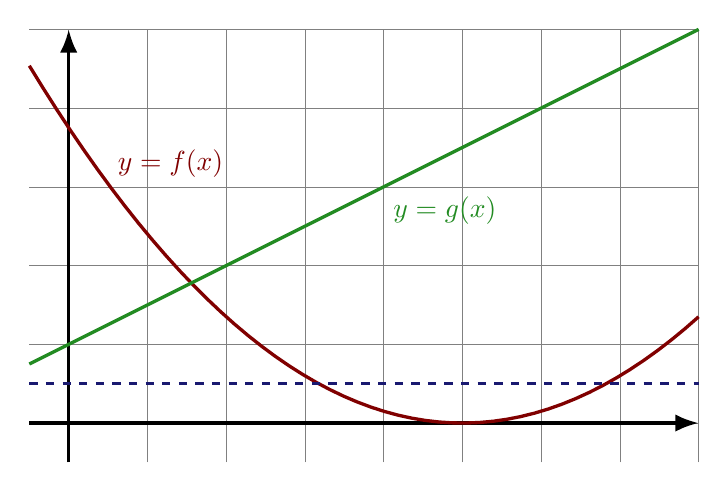
\begin{tikzpicture}
        \draw [help lines] (-0.5,-0.5) grid (8,5); 
        
        \draw [-Latex, very thick] (0, -0.5) -- (0, 5); 
        \draw [-Latex, very thick] (-0.5,0) -- (8,0); 
        
        \draw [Maroon, very thick, domain=-0.5:8, samples=50] plot (\x, 0.15*\x*\x-1.5*\x+3.75);
        \draw [ForestGreen, very thick, domain=-0.5:8] plot (\x, 0.5*\x + 1); 
        
        \node[Maroon, anchor=south west] at (0.5, 3) {\(y = f(x)\)};
        \node[ForestGreen, anchor=north west] at (4, 3) {\(y = g(x)\)};

        \draw [dashed, very thick, MidnightBlue] (-0.5, 0.5) -- (8, 0.5);
    \end{tikzpicture}
    \caption{The graphs of a non-injective function \(f(x)\) and an injective function \(g(x)\). The function \(g(x)\) is not injective because there exists a horizontal line (in blue) that intersects its graph at multiple points.}
    \label{fig:Ch3-injection-graph}
\end{figure}


There are a couple of ways to understand this definition intuitively:
\begin{itemize}
    \item In plain English, a function is injective when different inputs never share the same output. See figure \ref{fig:Ch3-injection}.
    \item Suppose the function is plotted on a coordinate system. A function is injective if there is no horizontal line that intersects its graph at more than one point. See figure \ref{fig:Ch3-injection-graph}.
\end{itemize}


\subsection{Surjections}

A function \(f : X \rightarrow Y\) is \textit{surjective} if its image is equal to its codomain, i.e.
%
\[\text{Image}(f) = Y\]
%
or
%
\[\forall y \in Y,\; \exists x \in X,\; f(x) = y\text{.}\]
%
Such a function is known as a \textit{surjection}.

\begin{figure}[H]
    \centering
    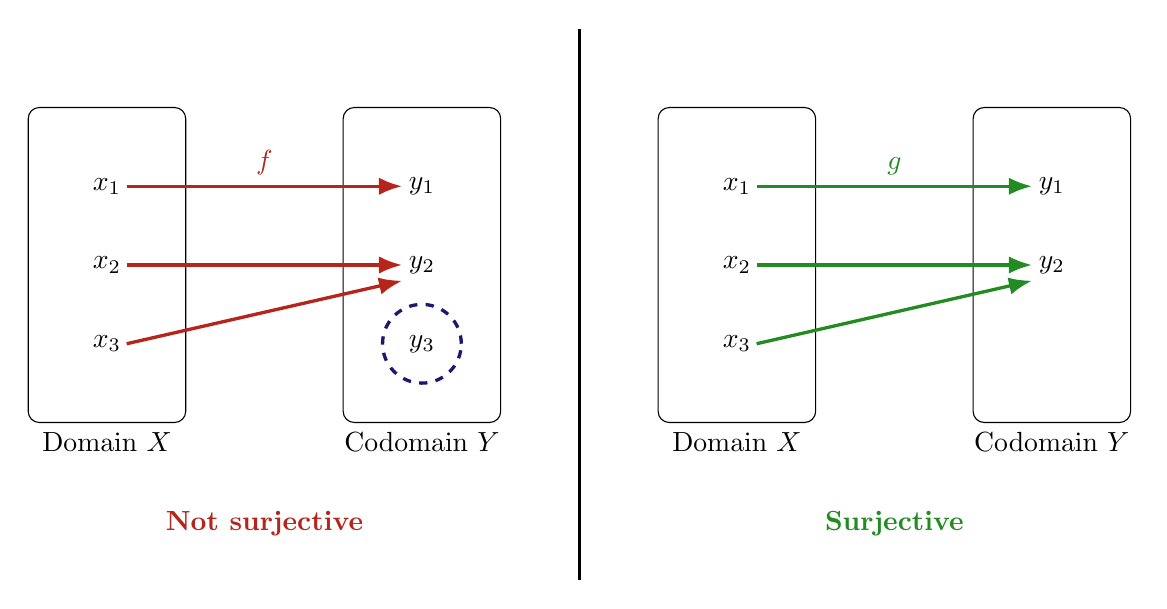
\begin{tikzpicture}
        \draw[rounded corners] (-3, 0) rectangle (-1, -4) {};
        \draw[rounded corners] (1, 0) rectangle (3, -4) {};

        \foreach \i  in {1,...,3} {
            \node[align=center, anchor=center] at (-2, -\i) {\(x_{\i}\)};
        }

        \foreach \i  in {1,...,3} {
            \node[align=center, anchor=center] at (2, -\i) {\(y_{\i}\)};
        }

        \draw[-Latex, very thick, BrickRed] (-1.75, -1) -- (1.75, -1) node[pos=0.5, anchor=south] {\(f\)};

        \node[anchor=north, BrickRed, align=left] at (0, -5) {\textbf{Not surjective}};

        \draw[-Latex, very thick, BrickRed] (-1.75, -2) -- (1.75, -2);

        \draw[-Latex, very thick, BrickRed] (-1.75, -3) -- (1.75, -2.2);

        \draw[MidnightBlue, very thick, dashed] (2,-3) circle [radius=0.5];

        \node[anchor=north] at (-2, -4) {Domain \(X\)};

        \node[anchor=north] at (2, -4) {Codomain \(Y\)};

        \draw[thick] (4, 1) -- (4, -6);
        
        \begin{scope}[shift={(8, 0)}]
            \draw[rounded corners] (-3, 0) rectangle (-1, -4) {};
            \draw[rounded corners] (1, 0) rectangle (3, -4) {};
    
            \foreach \i  in {1,...,3} {
                \node[align=center, anchor=center] at (-2, -\i) {\(x_{\i}\)};
            }
    
            \foreach \i  in {1,...,2} {
                \node[align=center, anchor=center] at (2, -\i) {\(y_{\i}\)};
            }
    
            \draw[-Latex, very thick, ForestGreen] (-1.75, -1) -- (1.75, -1) node[pos=0.5, anchor=south] {\(g\)};

            \draw[-Latex, very thick, ForestGreen] (-1.75, -3) -- (1.75, -2.2);

            \node[anchor=north, ForestGreen, align=left] at (0, -5) {\textbf{Surjective}};
            
            \draw[-Latex, very thick, ForestGreen] (-1.75, -2) -- (1.75, -2);
    
            \node[anchor=north] at (-2, -4) {Domain \(X\)};
    
            \node[anchor=north] at (2, -4) {Codomain \(Y\)};
        \end{scope}
        
    \end{tikzpicture}
    \caption{An non-surjective function \(f\) (left) and an surjective function \(g\) (right). The function \(f\) is not injective because its image is different from its codomain. The element \(y_3\), for example, is in the codomain but not in the image of \(f\).}
    \label{fig:Ch3-surjection}
\end{figure}


\subsection{Bijections (one-to-one correspondence)}

A function is \textit{bijective} if it is both surjective and injective. Such a function is said to have a \textit{one-to-one correspondence} between its inputs and its outputs.

For any bijective function \(f : X \rightarrow Y\), we define its \textit{inverse} as a function \(g : Y \rightarrow X\) such that:
%
\[
\begin{cases}
    g(f(x)) = x\\
    f(g(x)) = x
\end{cases}
\]

A function has an inverse if and only if it is bijective.

\begin{figure}[H]
    \centering
    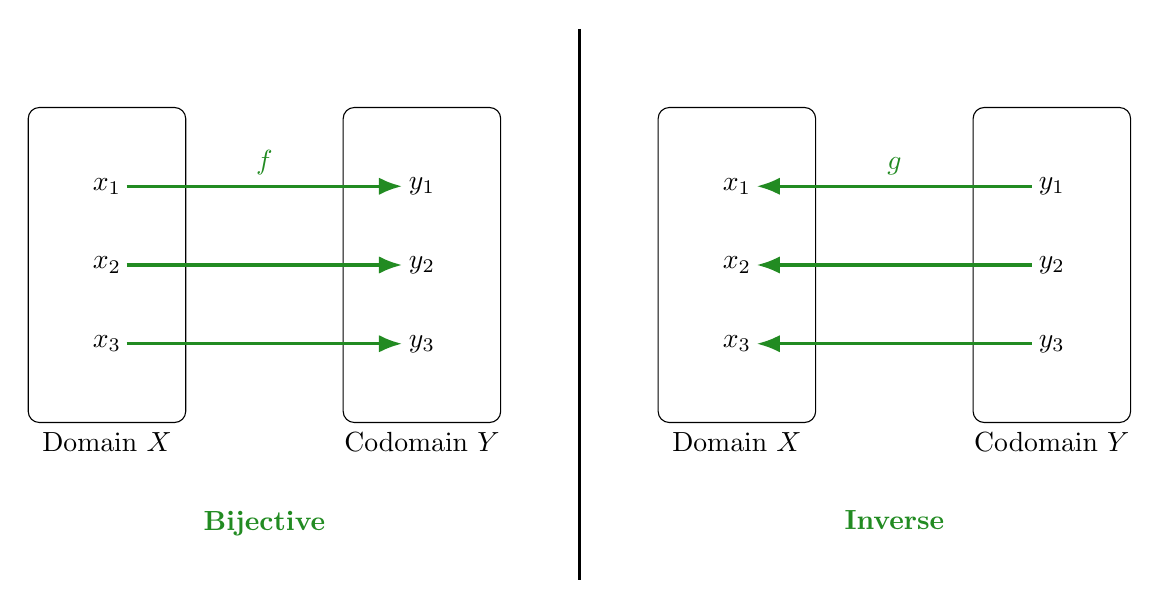
\begin{tikzpicture}
        \draw[rounded corners] (-3, 0) rectangle (-1, -4) {};
        \draw[rounded corners] (1, 0) rectangle (3, -4) {};

        \foreach \i  in {1,...,3} {
            \node[align=center, anchor=center] at (-2, -\i) {\(x_{\i}\)};
        }

        \foreach \i  in {1,...,3} {
            \node[align=center, anchor=center] at (2, -\i) {\(y_{\i}\)};
        }

        \draw[-Latex, very thick, ForestGreen] (-1.75, -1) -- (1.75, -1) node[pos=0.5, anchor=south] {\(f\)};

        \node[anchor=north, ForestGreen, align=left] at (0, -5) {\textbf{Bijective}};

        \draw[-Latex, very thick, ForestGreen] (-1.75, -2) -- (1.75, -2);

        \draw[-Latex, very thick, ForestGreen] (-1.75, -3) -- (1.75, -3);

        \node[anchor=north] at (-2, -4) {Domain \(X\)};

        \node[anchor=north] at (2, -4) {Codomain \(Y\)};

        \draw[thick] (4, 1) -- (4, -6);
        
        \begin{scope}[shift={(8, 0)}]
            \draw[rounded corners] (-3, 0) rectangle (-1, -4) {};
            \draw[rounded corners] (1, 0) rectangle (3, -4) {};
    
            \foreach \i  in {1,...,3} {
                \node[align=center, anchor=center] at (-2, -\i) {\(x_{\i}\)};
            }
    
            \foreach \i  in {1,...,3} {
                \node[align=center, anchor=center] at (2, -\i) {\(y_{\i}\)};
            }
    
            \draw[Latex-, very thick, ForestGreen] (-1.75, -1) -- (1.75, -1) node[pos=0.5, anchor=south] {\(g\)};
    
            \node[anchor=north, ForestGreen, align=left] at (0, -5) {\textbf{Inverse}};
    
            \draw[Latex-, very thick, ForestGreen] (-1.75, -2) -- (1.75, -2);
    
            \draw[Latex-, very thick, ForestGreen] (-1.75, -3) -- (1.75, -3);
    
            \node[anchor=north] at (-2, -4) {Domain \(X\)};
    
            \node[anchor=north] at (2, -4) {Codomain \(Y\)};
        \end{scope}
        
    \end{tikzpicture}
    \caption{A bijective function \(f\) (left) and its inverse (right).}
    \label{fig:Ch3-bijection-inverse}
\end{figure}



\subsection{Compositions of injections, surjections and bijections}

Given functions \(f : X \rightarrow Y\) and \(g : Y \rightarrow Z\), their composition \(h : X \rightarrow Z\) is given by \(h(x) = g(f(x))\).

We note the following properties.

\begin{enumerate}\setlength\itemsep{1.5em}
    \item \textbf{Composition of injections.}
    
    If \(f\) and \(g\) are both injective, then \(h\) is injective.

    \begin{proof}
        We want to show that for all \(a, b \in X\), if \(h(a) = h(b)\), then \(a = b\).
        
        Suppose \(h(a) = h(b)\) where \(a, b \in X\). It follows that
        %
        \begin{align*}
            g(f(a)) &= g(f(b))\\
            f(a) &= f(b) \tag{since \(g\) is injective}\\
            a &= b \tag{since \(f\) is injective}
        \end{align*}
        %
        Hence \(h\) is injective.
    \end{proof}

    \item \textbf{Composition of surjections.}
    
    If \(f\) and \(g\) are both surjective, then \(h\) is surjective.

    \begin{proof}
        We want to show that for any \(z \in Z\), there exists some \(x \in X\) such that \(h(x) = z\).

        Let \(z \in Z\). Since \(g\) is surjective, we know that
        \[\exists y \in Y,\; g(y) = z\text{.}\]
        %
        Also, since \(f\) is surjective,
        %
        \[\exists x \in X,\; f(x) = y\text{.}\]
        %
        Combining the two, we have
        %
        \begin{align*}
            \exists x \in X,&\; g(f(x)) = z\\
            \exists x \in X,&\; h(x) = z
        \end{align*}
        %
        Hence \(h\) is surjective.
    \end{proof}

    \item \textbf{Composition of bijections.}

    If \(f\) and \(g\) are both bijective, then \(h\) is bijective and has an inverse bijection \(h^{-1} : Z \rightarrow X\).

    \begin{proof}
        Since \(f\) and \(g\) are bijective, both of these functions are injective and surjective. It follows from the proofs above that \(h\) is both injective and surjective, so \(h\) is bijective.

        Also, since \(f\) and \(g\) are bijective, there exist functions \(f^{-1}\) and \(g^{-1}\) that are inverses to \(f\) and \(g\) respectively. We let \(h^{-1} = f^{-1} \circ g^{-1}\). Note that for any \(x \in X\),
        %
        \begin{align*}
            h^{-1} \circ h(x) &= f^{-1} \circ g^{-1} \circ g \circ f\\
            &= f^{-1} \circ f\\
            &= \text{id}_X
        \end{align*}
        %
        where \(\text{id}_X\) is the identity function on \(X\).
    \end{proof}
\end{enumerate}


\subsection{Proving the associativity of sequential composition of injections}

Given three injective functions \(f: A \rightarrow B\), \(g: B \rightarrow C\) and \(h: C \rightarrow D\), we can prove that their composition is associative:
%
\[(f; g); h = f; (g; h)\text{.}\]
%
This may seem obvious intuitively --- both sides tell us to apply \(f\), then \(g\), and then \(h\). Nonetheless we will provide a formal proof of this property below.
%
\begin{proof}
    For LHS, we have
    %
    \begin{align*}
        ({\color{BrickRed}(f; g)}; {\color{MidnightBlue} h})(x) &= {\color{MidnightBlue} h}({\color{BrickRed}(f; g)}(x))\\
        &= h(g(f(x)))\text{.}
    \end{align*}
    %
    Similarly for RHS we have
    %
    \begin{align*}
        ({\color{MidnightBlue} f}; {\color{BrickRed}(g; h)})(x) &= {\color{BrickRed}(g; h)}({\color{MidnightBlue} f}(x))\\
        &= h(g(f(x)))\text{.}
    \end{align*}
    %
    It follows that \(\text{LHS} = \text{RHS}\).
\end{proof}

\subsection{Comparing cardinalities of sets}

From figures \ref{fig:Ch3-injection} and \ref{fig:Ch3-bijection-inverse}, we can infer the following:
%
\begin{itemize}
    \item If there exists an injection \(f : X \rightarrow Y\), then \(\abs{Y} \geq \abs{X}\). (In addition, if there exists another injection \(g: Y \rightarrow X\), then \(\abs{X} \geq \abs{Y} \Rightarrow \abs{X} = \abs{Y}\).)
    \item If there exists a bijection \(f : X \rightarrow Y\), then \(\abs{Y} = \abs{X}\).
\end{itemize}
%
This generalizes to sets with an infinite number of elements.

The cardinality of the set of natural numbers is denoted as \(\abs{\mathbb{N}} = \aleph_0\) (``aleph-null''). If there exists a bijection between a set \(S\) and \(\mathbb{N}\) (i.e. \(\abs{S} = \abs{\mathbb{N}} = \aleph_0\)), then the set \(S\) is set to be \textit{countable} or \textit{enumerable}, because we can simply ``count'' the elements of \(S\) with natural numbers. Here are a couple of examples.

\begin{enumerate}\setlength\itemsep{1.5em}
    \item \textbf{\(\mathbb{Z}\) is countable.}
    
    \begin{proof}
        For each \(n \in \mathbb{Z}\) we define \(f : \mathbb{Z} \rightarrow \mathbb{N}\) as follows.
        %
        \[f(n) = \begin{cases}
            2n \hspace{2.75em}\text{(for \(n>0\))}\\
            -2n+1 \;\;\text{(for \(n \leq 0\))}
        \end{cases}\]
        %
        This function is bijective as it has an inverse:
        %
        \[f^{-1}(m) = \begin{cases}
            m/2 \hspace{2.75em}\text{(if \(m\) is even)}\\
            (1-m)/2 \;\;\text{(if \(m\) is odd)}
        \end{cases}\]
    \end{proof}

    \begin{figure}[H]
        \centering
        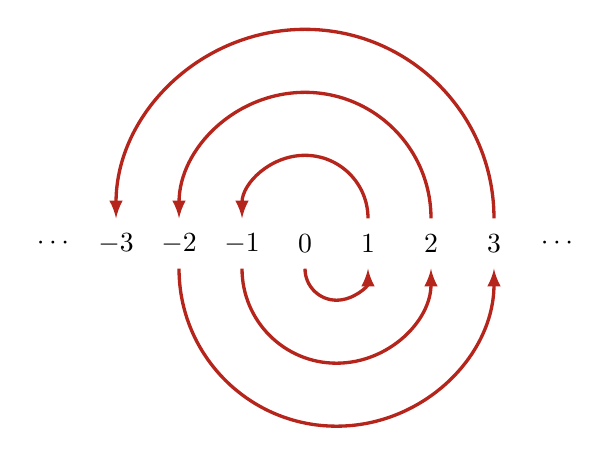
\begin{tikzpicture}[scale=0.8]
            \foreach \x in {-4, ..., 4} {
                \ifthenelse{\x=4 \OR \x=-4}{
                    \node at (\x,0) {\(\cdots\)};
                }{
                    \node at (\x,0) {\(\x\)};
                }
            }

            \foreach \x in {1, 2, 3} {
                \draw[-latex, very thick, BrickRed] (1-\x, -0.4) arc (180:360:\x-0.5);

                \draw[-latex, very thick, BrickRed] (\x, 0.4) arc (0:180:\x);
            }
        \end{tikzpicture}
        \caption{Counting through the set of integers.}
        \label{fig:ch3-counting-through-z}
    \end{figure}

    
    \item \textbf{\(\mathbb{N} \times \mathbb{N}\) is countable.}

    \begin{proof}
        Arrange the ordered pairs \((m, n)\) where \(m, n \in \mathbb{N}\) in a table like so.

        \begin{figure}[H]
            \centering
            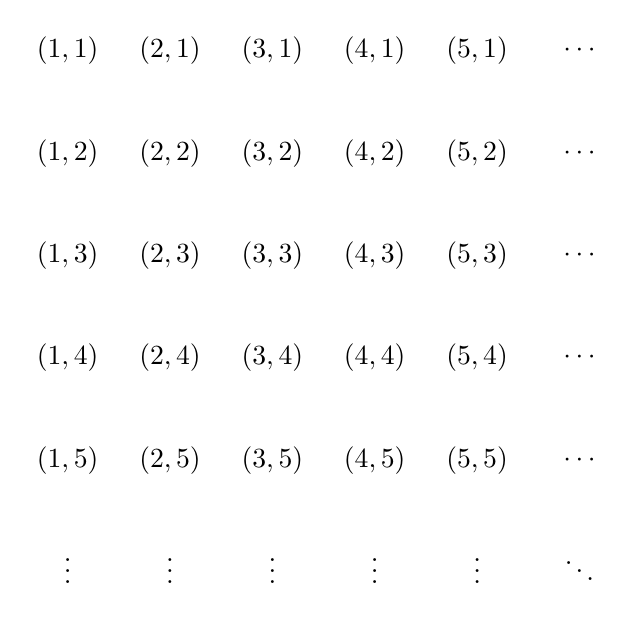
\begin{tikzpicture}[scale=1.3]
                \foreach \x in {1, ..., 6} {
                    \foreach \y in {1, ..., 6} {
                        \ifthenelse{\x=6 \AND \y=6}{
                            \node at (\x,-\y) {\(\ddots\)};
                        }{
                            \ifthenelse{\x=6}{
                                \node at (\x,-\y) {\(\cdots\)};
                            }{
                                \ifthenelse{\y=6}{
                                    \node at (\x,-\y) {\(\vdots\)};
                                }{
                                    \node at (\x,-\y) {\((\x,\y)\)};
                                }
                            }
                        }
                    }
                }
            \end{tikzpicture}
            \caption{A grid of ordered pairs \((m, n)\) where \(m, n \in \mathbb{N}\).}
            \label{fig:ch3-grid-of-ordered-pairs}
        \end{figure}

        We can then count them as follows.

        \begin{figure}[H]
            \centering
            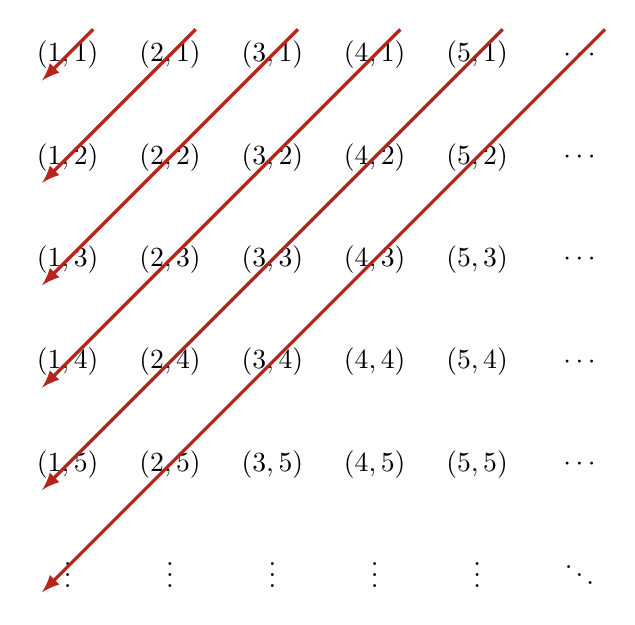
\begin{tikzpicture}[scale=1.3]
                \foreach \x in {1, ..., 6} {
                    \foreach \y in {1, ..., 6} {
                        \ifthenelse{\x=6 \AND \y=6}{
                            \node at (\x,-\y) {\(\ddots\)};
                        }{
                            \ifthenelse{\x=6}{
                                \node at (\x,-\y) {\(\cdots\)};
                            }{
                                \ifthenelse{\y=6}{
                                    \node at (\x,-\y) {\(\vdots\)};
                                }{
                                    \node at (\x,-\y) {\((\x,\y)\)};
                                }
                            }
                        }
                    }
                }

                \foreach \i in {1, ..., 6} {
                    \draw[BrickRed, very thick, -latex] (\i + 0.25, -1+0.25) -- (1-0.25, -\i-0.25);
                }
            \end{tikzpicture}
            \caption{Counting through ordered pairs of natural numbers.}
            \label{fig:ch3-counting-through-ordered-pairs}\qedhere
        \end{figure}
    \end{proof}

    The same argument above can be modified to show that the set of rational numbers \(\mathbb{Q}\) is countable.
\end{enumerate}

Note that not all infinite sets are countable. The set of real numbers, for example, is uncountable as its cardinality exceeds \(\aleph_0\).

\newpage
\section{Permutations}

\subsection{What is a permutation?}

A \textit{permutation} is an order in which a set of elements can be arranged. A permutation involving \(n\) elements is said to have \textit{degree} \(n\). In general, as we know from combinatorics, there are \(n!\) permutations of degree \(n\).

For instance, the integers 1, 2 and 3 can be arranged in 6 different ways, each of which is considered a different permutation of degree 3.
%
\begin{center}
    (1, 2, 3)\\
    (1, 3, 2)\\
    (2, 1, 3)\\
    (2, 3, 1)\\
    (3, 1, 2)\\
    (3, 2, 1)
\end{center}
%
We can denote each of these permutations using the following two-line notation.
%
\begin{alignat*}{5}
&
\begin{pmatrix}
    1 & 2 & 3\\
    1 & 2 & 3
\end{pmatrix}
&&\;\;&&
\begin{pmatrix}
    1 & 2 & 3\\
    1 & 3 & 2
\end{pmatrix}
&&\;\;&&
\begin{pmatrix}
    1 & 2 & 3\\
    2 & 1 & 3
\end{pmatrix}
\\&&&&&&&&&\\
&
\begin{pmatrix}
    1 & 2 & 3\\
    2 & 3 & 1
\end{pmatrix}
&&&&
\begin{pmatrix}
    1 & 2 & 3\\
    3 & 1 & 2
\end{pmatrix}
&&&&
\begin{pmatrix}
    1 & 2 & 3\\
    3 & 2 & 1
\end{pmatrix}
\end{alignat*}


\subsection{Viewing permutations as bijections}

Looking at the two-line notation, one might notice that any given permutation is merely a bijective function in disguise. For example, the permutation 
%
\[
\begin{pmatrix}
    1 & 2 & 3\\
    3 & 1 & 2
\end{pmatrix}
\]
%
can be represented by a bijective function \(\sigma : \{1, 2, 3\} \rightarrow \{1, 2, 3\}\), where
%
\[
\begin{cases}
    \sigma(1) = 3\\
    \sigma(2) = 1\\
    \sigma(3) = 2\text{.}
\end{cases}
\]
%
In fact, we can define a permutation of degree \(n\) to be a bijection \(\sigma : \{1, 2, 3, \cdots, n\} \rightarrow \{1, 2, 3, \cdots, n\}\). We also define the \textit{symmetric group} of degree \(n\), denoted as \(S_n\), to be the set of all permutations of degree \(n\).

For example, the symmetric group of degree 3 has the following elements.
%
\[
S_3 = \left\{
\begin{pmatrix}
    1 & 2 & 3\\
    1 & 2 & 3
\end{pmatrix},
%
\begin{pmatrix}
    1 & 2 & 3\\
    1 & 3 & 2
\end{pmatrix},
%
\begin{pmatrix}
    1 & 2 & 3\\
    2 & 1 & 3
\end{pmatrix},
%
\begin{pmatrix}
    1 & 2 & 3\\
    2 & 3 & 1
\end{pmatrix},
%
\begin{pmatrix}
    1 & 2 & 3\\
    3 & 1 & 2
\end{pmatrix},
%
\begin{pmatrix}
    1 & 2 & 3\\
    3 & 2 & 1
\end{pmatrix}
\right\}
\]

Now, consider the permutation
%
\[\epsilon = \begin{pmatrix}
    1 & 2 & 3\\
    1 & 2 & 3
\end{pmatrix}\text{.}\]
%
As the order of the elements is unchanged, this bijection is simply the identity function. Such a permutation, where \(\forall k \in \{1, 2, 3, \cdots, n\}, \epsilon(k) = k\), is called an \textit{identity permutation}.


\subsection{Composition and order of permutations}

Viewing permutations as bijections allows us to composite permutations in the same way that we composite functions. An example of this is displayed below.

\begin{figure}[H]
    \centering
    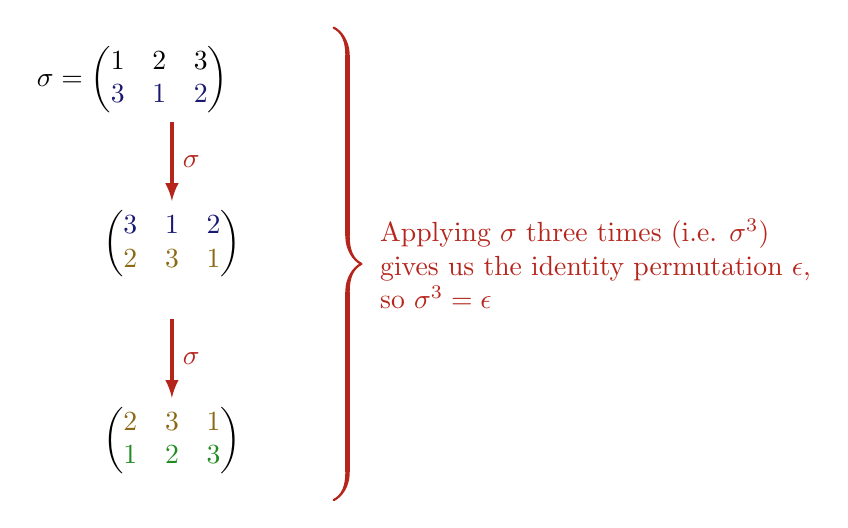
\begin{tikzpicture}    
        \node[align=center, anchor=south] at (-0.5, 0) {\(
            \sigma =
            \begin{pmatrix}
                1 & 2 & 3\\
                {\color{MidnightBlue} 3} & {\color{MidnightBlue} 1} &{\color{MidnightBlue} 2}
            \end{pmatrix}
        \)};

        \draw[very thick, -latex, BrickRed] (0, 0) -- (0, -1) node[pos=0.5, anchor=west]{\(\sigma\)};

        \node[align=center, anchor=north] at (0, -1) {\(
            \begin{pmatrix}
                {\color{MidnightBlue} 3} & {\color{MidnightBlue} 1} &{\color{MidnightBlue} 2}\\

                {\color{Goldenrod4} 2} & {\color{Goldenrod4} 3} &{\color{Goldenrod4} 1}
            \end{pmatrix}
        \)};

        \draw[very thick, -latex, BrickRed] (0, -2.5) -- (0, -3.5) node[pos=0.5, anchor=west]{\(\sigma\)};

        \node[align=center, anchor=north] at (0, -3.5) {\(
            \begin{pmatrix}
                {\color{Goldenrod4} 2} & {\color{Goldenrod4} 3} &{\color{Goldenrod4} 1}\\

                {\color{ForestGreen} 1} & {\color{ForestGreen} 2} &{\color{ForestGreen} 3}
            \end{pmatrix}
        \)};

        \draw[pen colour={BrickRed}, decoration={calligraphic brace, amplitude=10pt, raise=30pt},decorate, ultra thick] (1,1.2) -- (1,-4.8) node[pos=0.5, anchor=west, BrickRed, align=left, shift={(1.5, 0)}] {Applying \(\sigma\) three times (i.e. \(\sigma^3\))\\ gives us the identity permutation \(\epsilon\),\\ so \(\sigma^3 = \epsilon\)};
    \end{tikzpicture}
    \caption{An example of compositing permutations.}
    \label{fig:ch4-permutation-composition}
\end{figure}


We define the \textit{order} of a permutation \(\sigma\) to be the smallest positive integer \(k\) such that \(\sigma^k = \epsilon\), where \(\epsilon\) is the identity permutation. For example, in figure \ref{fig:ch4-permutation-composition}, applying \(\sigma\) three times takes us back to the start. This means that \(\sigma^3 = \epsilon\), the order of \(\sigma\) is 3.


\subsection{Disorders, and the sign of a permutation}\label{sec:sign-of-permutation}

For any given permutation \(\sigma\), a \textit{disorder} is a pair of values \((x, y)\) where \(x < y\) but \(\sigma(x) > \sigma(y)\).

If a permutation has an even number of disorders, then it is said to have a sign of \(+1\). If the number of disorders is odd, then the permutation has a sign of \(-1\).

For example, the permutation
%
\[
\sigma =
\begin{pmatrix}
    1 & 2 & 3\\
    3 & 1 & 2
\end{pmatrix}
\text{,}
\]
%
has two disorders: \((3, 1)\) and \((3, 2)\). Therefore, its sign must be \(\sgn(\sigma) = +1\).

Note that the sign of a permutation is defined in such a way that for any two permutations \(\sigma_1\) and \(\sigma_2\), we have
%
\[\sgn(\sigma_1 \sigma_2) = \sgn(\sigma_1) \cdot \sgn(\sigma_2)\text{.}\]


\newpage
\section{Introduction to modular arithmetic}

Consider the integer division \(100 \div 7\), which produces the quotient 14 and remainder 2 (because \(100 = 7 \times 14 + 2\)).

Since this division produces the remainder 2, we say that 100 \textit{modulo} 7 is equal to 2. This is denoted as \(100 \bmod 7 = 2\). The divisor (which is 7 in this case) is known as the \textit{modulus}.

Note the following facts about the modulo operator:
%
\begin{itemize}
    \item For a given modulus \(m\), the remainder must be an integer inclusively between 0 and \(m - 1\). This gives us the set of remainders \(G_m = \{0, 1, 2, \cdots, m-2, m-1\}\).
    
    \item If two integers \(a\) and \(b\) differ by a multiple of \(m\), they must produce the same remainder when divided by \(m\). When this happens, we say that \(a\) and \(b\) are congruent modulo \(m\). This is denoted as \(a \equiv b \pmod m\).

    \item We can perform addition and multiplication on the set of remainders. If \(a_1 = a_2 \pmod m\) and \(b_1  = b_2 \pmod m\), then:
    \begin{align*}
        a_1 + b_1 &= a_2 + b_2 \pmod m\\
        a_2 \cdot b_2 &= a_2 \cdot b_2 \;\;\pmod m
    \end{align*}
    As an example, the addition and multiplication tables for the modulus 4 is shown below.

    \begin{table}[H]
        \centering
        \begin{tabular}{|c|cccc|}
            \hline
            \(+ \pmod 4\) & 0 & 1 & 2 & 3\\
            \hline
            0 & 0 & 1 & 2 & 3\\
            1 & 1 & 2 & 3 & 0\\
            2 & 2 & 3 & 0 & 1\\
            3 & 3 & 0 & 1 & 2\\
            \hline
        \end{tabular}
        \caption{Addition on the set of remainders modulo 4.}
        \label{tab:ch5-plus-mod4}
    \end{table}

    \begin{table}[H]
        \centering
        \begin{tabular}{|c|cccc|}
            \hline
            \(\times \pmod 4\) & 0 & 1 & 2 & 3\\
            \hline
            0 & 0 & 0 & 0 & 0\\
            1 & 0 & 1 & 2 & 3\\
            2 & 0 & 2 & 0 & 2\\
            3 & 0 & 3 & 2 & 1\\
            \hline
        \end{tabular}
        \caption{Multiplication on the set of remainders modulo 4.}
        \label{tab:ch5-times-mod4}
    \end{table}
\end{itemize}

We will talk more about modular arithmetic in the following chapters.

\newpage
\section{Binary relations}

\subsection{What is a binary relation?}

A \textit{binary relation} \(R(x, y)\) describes some relationship between \(x\) and \(y\) where \(x \in X\), \(y \in Y\) and \(R \subseteq X \times Y\). Examples include:
%
\begin{itemize}
    \item ``\(x < y\)''.
    \item ``\(y = x^2\)''.
    \item ``\(x\) is a child of \(y\)''.
    \item ``\(x\) and \(y\) are students from the same school''.
\end{itemize}


\subsection{Equivalence relations}

A binary relation is said to be an \textit{equivalence relation} on the set \(X\) if and only if it satisfies all of the following conditions.
%
\begin{enumerate}
    \item \textbf{Reflexivity:} Any element in \(X\) must be considered equivalent to itself.
    \[\forall x \in X,\; E(x, x)\]

    \item \textbf{Symmetry:} If \(x\) is considered equivalent to \(y\), then \(y\) must also be considered equivalent to \(x\).
    \[\forall x, y \in X,\; E(x, y) \Leftrightarrow E(y, x)\]

    \item \textbf{Transitivity:} If \(x\) is considered equivalent to \(y\), and \(y\) is considered equivalent to \(z\), then it follows that \(x\) must be considered equivalent to \(z\).
    \[\forall x, y, z \in X,\; E(x, y) \wedge E(y, z) \Rightarrow E(x, z)\]
\end{enumerate}

Examples of equivalence relations include
\begin{itemize}
    \item ``is equal to'' on the set of numbers;
    \item ``is similar to'' on the set of all triangles; and
    \item ``is congruent to, mod \(m\)'' on the set of integers.
\end{itemize}


\subsection{Equivalence classes}

Suppose we have an equivalence relation \(E(x, y)\) acting on a set \(X\). For any element \(a \in X\), we define its \textit{equivalence class} \([a]\) as the set of all elements in \(X\) that are considered ``equivalent'' to \(a\):
%
\[[a] := \{x \in X \setvert E(x, a)\}\]
%
Note that by definition \([a]\) is a subset of \(X\).

For example, consider the equivalence relation ``\(x - y\) is even'' which acts on the set of all integers. This gives us the following equivalence classes for 0 and 1.
%
\begin{align*}
    [0] &= \{0, 2, -2, 4, -4, \cdots, 2n, -2n, \cdots\}\\
    [1] &= \{1, -1, 3, -3, \cdots, 2n+1, -2n-1, \cdots\}
\end{align*}



\newpage
\section{Introduction to groups}

\subsection{What is a group?}

Consider a nonempty set \(G\) and a binary operation \(* : G \times G \rightarrow G\). The pair \((G, *)\) is said to be a \textit{group} if and only if it has the following properties.
%
\begin{enumerate}
    \item \textbf{Closure:} For any two elements \(x\) and \(y\) in \(G\), the value \(x * y\) must also be an element of \(G\).
    \[\forall x, y \in G,\; x * y \in G\]

    \item \textbf{Associativity:} If we want to repeatedly perform the operation \(*\) on three elements in \(G\), it doesn't matter where we put the brackets.
    \[\forall x, y, z \in G,\; (x*y)*z = x*(y*z)\]

    \item \textbf{Existence of identity element:} There is a unique \textit{identity element} \(\epsilon\) in \(G\) such that performing the operation \(*\) on \(x\) with \(\epsilon\) (in any order) should give us the value of \(x\) back.
    %
    \[\exists \epsilon \in G,\; \forall x \in G,\; x * \epsilon = \epsilon * x = x\]
    %
    The identity element is sometimes called the \textit{neutral element}, or simply the \textit{identity}.

    \item \textbf{Invertibility (i.e. existence of inverse for all elements):} For any element \(x\) in \(G\), there exists a corresponding unique \textit{inverse} element \(x^{-1}\) in \(G\) such that performing the operation \(*\) on \(x\) with \(x^{-1}\) (in any order) produces the identity element.
    %
    \[\forall x \in G,\; \exists x^{-1} \in G,\; x * x^{-1} = x^{-1} * x = \epsilon\]
    %
    Note that \(x^{-1}\) refers merely to the inverse of \(x\), and does not necessarily denote the reciprocal of \(x\).
\end{enumerate}

The \textit{order} of a group \((G, *)\) is defined as the cardinality of the set \(G\).


\subsection{Commutative groups}

Occasionally, a group \((G, *)\) might happen to satisfy a fifth, additional condition --- commutativity. This means that if we want to perform the operation \(*\) on two elements \(x\) and \(y\), it doesn't matter what order we put the two elements in.
%
\[\forall x, y \in G,\; x * y = y * x\]
%
This kind of group is called a \textit{commutative group}.


\subsection{Additive groups}

The operation of a group can be anything as long as it's binary; but we also have special names for groups with specific operations. For example, a group with addition as its operation is known as an \textit{additive group}.

\((\mathbb{Z}, +)\) is an example of an additive group. It satisfies closure (the sum of any two integers is also an integer) and associativity (\((x + y) + z = x + (y + z)\)); it has an identity element (\(\epsilon = 0\)), and every element \(x\) has a corresponding unique inverse \(x^{-1} = -x\) where \(x + (-x) = 0\).

As addition is commutative, this is also a commutative group.

The group \((\mathbb{Z}, +)\) has the following property:
%
\begin{quote}
    For any two integers \(a\) and \(b\), the equation \(a + z = b\) has a unique solution.
    %
    \begin{proof}
    We start by showing the existence of such a solution. By setting \(z = -a + b\), we have:
    \begin{align*}
        a + z &= a + ((-a) + b)\\
        &= (a + (-a)) + b \tag{associativity}\\
        &= 0 + b\\
        &= b
    \end{align*}
    %
    which implies that \(z = -a + b\) is a solution to the aforementioned equation.

    To show that this solution is unique, suppose \(z_1\) and \(z_2\) are both integers that satisfy the equation.
    %
    \[
    \begin{cases}
        a + z_1 = b\\
        a + z_2 = b
    \end{cases}
    \]
    %
    We then add the inverse of \(a\), or \(-a\), to both sides of each equation.
    %
    \[
    \begin{cases}
        (-a) + a + z_1 = -a + b\\
        (-a) + a + z_2 = -a + b
    \end{cases}
    \]
    %
    Since \((-a)+a = 0\), this gives us the following set of equations:
    %
    \[
    \begin{cases}
        z_1 = -a + b\\
        z_2 = -a + b
    \end{cases}
    \]
    %
    which gives \(z_1 = -a+b = z_2\). This means that \(z = -a+b\) is indeed a unique solution to the equation.
    \end{proof}
\end{quote}

This property holds for all other additive groups as well.

Another additive group is the group formed by the set of remainders \(G_m = \{0, 1, 2, \cdots, m-2, m-1\}\) with respect to addition modulo \(m\). We can once again check that it satisfies closure and associativity, with the existence of an identity element (0) and an inverse for every element in \(G_m\).

We note that \((\mathbb{N}, +)\) is \textit{not} a group as not all elements have inverses. For instance, for the element 2, there is no \(n \in \mathbb{N}\) that satisfies \(n + 2 = \epsilon = 0\).


\subsection{Multiplicative groups}

Similar to what we saw above, a group with multiplication as its operation is known as an \textit{multiplicative group}.

An example of a multiplicative group is \((\mathbb{R}^{+}, \times)\). Again, we can easily verify that it satisfies all four prerequisites for a group --- the identity element is 1, and each element \(x \in \mathbb{R}^+\) has \(x^{-1} = 1/x\) as its inverse --- and that it has the bonus property of commutativity. Moreover, we can prove the following theorem, similar to the previous one we proved for additive groups.
%
\begin{quote}
    For any two positive real numbers \(a\) and \(b\), the equation \(a \times z = b\) has a unique solution.
    %
    \begin{proof}
    We start by showing the existence of such a solution. By setting \(z = 1/a \times b\), we have:
    \begin{align*}
        a \times z &= a \times (1/a \times b)\\
        &= (a \times 1/a) \times b \tag{associativity}\\
        &= 1 \times b\\
        &= b
    \end{align*}
    %
    which means \(z = 1/a + b\) is a solution to the equation.

    To show that this solution is unique, suppose \(z_1\) and \(z_2\) are both positive real numbers that satisfy the equation.
    %
    \[
    \begin{cases}
        a \times z_1 = b\\
        a \times z_2 = b
    \end{cases}
    \]
    %
    We then multiply the inverse of \(a\), or \(1/a\), on both sides of each equation.
    %
    \[
    \begin{cases}
        1/a \times a \times z_1 = 1/a \times b\\
        1/a \times a \times z_2 = 1/a \times b
    \end{cases}
    \]
    %
    Since \(1/a \times a = 1\), this gives us the following set of equations:
    %
    \[
    \begin{cases}
        z_1 = 1/a \times b\\
        z_2 = 1/a \times b
    \end{cases}
    \]
    %
    which gives \(z_1 = 1/a \times b = z_2\). This means that \(z = 1/a \times b\) is indeed a unique solution to the equation.
    \end{proof}
\end{quote}

This property holds for all other multiplicative groups too.

As a sidenote, the group formed by the set of permutations of degree \(n\) with respect to multiplication (i.e. composition) is also a multiplicative group.


\subsection{Subgroups}

Given a group \((G, *)\), if there exists a subset \(H \subseteq G\) such that \((H, *)\) too fulfills closure, has a neutral element and has invertibility, then \((H, *)\) is said to be a \textit{subgroup} of \((G, *)\).

Note that
\begin{itemize}
    \item Associativity is not listed above because if the operation \(*\) is associative for all elements of \(G\), it must also be associative for all elements of \(H\).
    \item Although the term ``subgroup'' refers to \((H, *)\), in casual usage, mathematicians may sometimes use the word ``subgroup'' when only referring to the subset \(H\).
\end{itemize}

For any group \((G, *)\), let \(a\) be an element of \(G\). We can use \(a\) to generate a subgroup \((H, *)\) like so:
%
\[H = \{a^k \setvert k \in \mathbb{Z}\} = \{\cdots, a^{-2}, a^{-1}, a^0, a^1, a^2, \cdots\}\]
%
where
\begin{itemize}
    \item \(a^{-k} = \underbrace{a^{-1} * a^{-1} * \cdots * a^{-1}}_{\text{\(k\) times}}\);
    \item \(a^{0} = \epsilon\); and
    \item \(a^{k} = \underbrace{a * a * \cdots * a}_{\text{\(k\) times}}\).
\end{itemize}
%
Such a subgroup is called a \textit{cyclic subgroup}.

As an example, consider the multiplicative group \((\mathbb{C}, \times)\). A cyclic subgroup of this group can be formed with the set \(\{i, i^2, i^3, i^4\} = \{i, -1, -i, 1\}\) as it satisfies closure, has the neutral element \(1\) and has inverses for each element.


\subsection{Order of an element}

Given a group \((G, *)\), we define the \textit{order} of an element \(a \in G\) as the smallest positive integer \(k\) such that \(a^k = \epsilon\), where \(\epsilon\) is the identity element.

This is not to be confused with the order of a group, which refers to the cardinality of \(G\).

\newpage
\section{Euclidean algorithm and its applications in groups}

\subsection{Multiplicative group of integers modulo \(m\)}

Here we take a look at a special kind of multiplicative group. For any modulus \(m\), we define the \textit{multiplicative group of integers modulo \(m\)} as the group formed by the set
%
\[G^{\times}_m = \{a \setvert (1 \leq a < m) \wedge (\gcd{(a, m)} = 1)\}\]
%
with respect to multiplication \(\bmod{\;m}\).

Put plainly, the set \(G^{\times}_m\) is simply the set of all integers inclusively between \(1\) and \((m - 1)\) that are coprime with \(m\). For example, the multiplicative group of integers modulo \(15\) is \(G^{\times}_{15} = \{1, 2, 4, 7, 8, 11, 13, 14\}\).


\subsection{Euler's totient function}

For any positive integer \(m\), we define \textit{Euler's totient function} \(\phi(m)\) as the cardinality of the set \(G^{\times}_m\), i.e.
%
\[\phi(m) = \abs{G^{\times}_m}\text{.}\]
%
This allows us to say something like \(\phi(15) = 8\), because between 1 and 15 (inclusive), there are 8 integers that are coprime with 15.

% For any prime \(p\), we have \(\gcd{(p, n)} = 1\) for any positive integer \(n\). Hence, \(\phi(p) = p-1\).

Let us investigate the properties of this function. In particular, we want to answer these two questions:
%
\begin{enumerate}
    \item If a certain number \(p\) is prime, what does that tell us about \(\phi(p)\)?

    \item Now suppose we have two primes \(p\) and \(q\). What does that tell us about \(\phi(pq)\)?
\end{enumerate}

The first question is easy. Since \(p\) is prime, we have \(G^\times_p = \{1, 2, 3, \cdots, p-2, p-1\}\), which gives us \(\phi(p) = p-1\).

Answering the second question requires a change in perspective. Instead of thinking ``how many numbers are in \(G^\times_{pq}\)'', it might be more helpful to think ``how many numbers are \textit{not} in \(G^\times_{pq}\)''. There are a total of \(pq\) integers from 1 to \(pq\), and among these integers,
%
\begin{itemize}
    \item There are \(p\) multiples of \(q\):
    %
    \[q,\; 2q,\; 3q,\; \cdots,\; pq\]
    %
    Each of these multiples shares a common divisor of \(q\) with \(pq\), and thus will not appear in the set \(G^\times_{pq}\).

    \item Similarly, there are \(q\) multiples of \(p\):
    %
    \[p,\; 2p,\; 3p,\; \cdots,\; pq\]
    %
    Each of these multiples shares a common divisor of \(p\) with \(pq\), and therefore will not appear in the set \(G^\times_{pq}\) either.
\end{itemize}
%
Since both \(p\) and \(q\) are prime, these are the only integers from 1 to \(pq\) that do not appear in \(G^\times_{pq}\). Taking into account the fact that \(pq\) is double-counted in the two cases above, we can calculate \(\phi(pq) = \abs{G^\times_{pq}}\) as follows.
%
\begin{align*}
    \phi(pq) &= \abs{G^\times_{pq}}\\
    &= (\text{\# of integers from \(1\) to \(pq\)}) - (\text{\# of non-coprime integers from \(1\) to \(pq\)})\\
    &= pq - ((\text{\# of multiples of \(q\)}) + (\text{\# of multiples of \(p\)}) - 1)\\
    &= pq - (p + q - 1)\\
    &= pq - p - q + 1\\
    &= (p-1)(q-1)\\
    &= \phi(p)\cdot \phi(q)
\end{align*}

This conclusion that \(\phi(pq) = \phi(p)\cdot \phi(q) = (p-1)(q-1)\) can be very useful when calculating \(\phi(pq)\) for relatively large values of \(p\) and \(q\). For example, to compute \(\phi(143)\), we can break 143 down into two primes, giving us
%
\begin{align*}
    \phi(143) &= \phi(11 \times 13)\\
    &= \phi(11) \times \phi(13)\\
    &= (11-1)(13-1)\\
    &= 120\text{.}
\end{align*}


\subsection{But is it really a group?}

To verify that the set \(G^{\times}_m\) indeed forms a group with respect to multiplication \(\pmod{m}\), we must check if it satisfies the four criteria outlined in the previous section.
%
\begin{itemize}
    \item \textbf{Closure.} Since \((\gcd(a, m) = 1) \wedge (\gcd(b, m) = 1) \Rightarrow \gcd(a\times b, m) = 1\), this group satisfies closure.
    \item \textbf{Associativity.} Multiplication is associative.
    \item \textbf{Existence of identity element}. For any element \(a \in G^{\times}_{m}\), we have \(a \cdot 1 = 1 \cdot a = a\), so \(1\) is the identity element for this group.
    \item \textbf{Existence of inverse for all elements.} For any \(a \in G^{\times}_m\) we can find some \(a^{-1}\) from \(G^{\times}_m\) such that \(a \times a^{-1} = 1 \pmod{m}\). (Or can we?)
\end{itemize}
%
The last criterion, invertibility, is slightly more difficult to prove. To show that \((G^{\times}_m, \times)\) fulfils this condition, we will first have to introduce the Euclidean algorithm.


\subsection{Euclidean algorithm}

Given two integers \(a\) and \(b\) (where \(a > b\) without loss of generality), the Euclidean algorithm (or Euclid's algorithm) can be used to compute their greatest common divisor \(\gcd{(a, b)}\).

It's best to illustrate the algorithm with an example. Suppose we want to evaluate the greatest common divisor between the numbers 600 and 11312. To do this, we divide the larger number by the smaller one to get a quotient and a remainder.

\begin{tabular}{c|c}
    \parbox{0.5\textwidth}{\centering
        \(11312 = 18 \times 600 + 512\)
    }
    &
    \parbox{0.5\textwidth}{\centering
        \(a = 18 \times b + r_1\)
    }
\end{tabular}

Ignoring the quotient, we take the two numbers on the RHS (600 and 512) and perform integer division on them again.

\begin{tabular}{c|c}
    \parbox{0.5\textwidth}{\centering
        \(600 = 1 \times 512 + 88\)
    }
    &
    \parbox{0.5\textwidth}{\centering
        \(b = 1 \times r_1 + r_2\)
    }
\end{tabular}

We repeat this process until we get a remainder of 0.

\begin{tabular}{c|c}
    \parbox{0.5\textwidth}{\centering
        \begin{align*}
            512 &= 5 \times 88 + 72\\
            88 &= 1 \times 72 + 16\\
            72 &= 4 \times 16 + 8\\
            16 &= 2 \times 8 + 0
        \end{align*}
    }
    &
    \parbox{0.5\textwidth}{\centering
        \begin{align*}
            r_1 &= 5 \times r_2 + r_3\\
            r_2 &= 1 \times r_3 + r_4\\
            r_3 &= 4 \times r_4 + r_5\\
            r_4 &= 2 \times r_5 + 0
        \end{align*}
    }
\end{tabular}

The GCD of the two original numbers is the last nonzero remainder obtained, which in this case is \(r_5 = 8\).

As another example, here is a demonstration of the Euclidean algorithm with the numbers \(a = 408\) and \(b = 126\).

\begin{tabular}{c|c}
    \parbox{0.5\textwidth}{\centering
        \begin{align*}
            408 &= 3 \times 126 + 30\\
            126 &= 4 \times 30 + 6\\
            30 &= 5 \times 6 + 0
        \end{align*}
    }
    &
    \parbox{0.5\textwidth}{\centering
        \begin{align*}
            a &= 3 \times b + r_1\\
            b &= 4 \times r_1 + r_2\\
            r_1 &= 5 \times r_2 + 0
        \end{align*}
    }
\end{tabular}

The result here is \(\gcd{(408, 126)} = r_2 = 6\).


\subsection{Expressing \(\gcd{(a, b)}\) as a linear combination of \(a\) and \(b\)}

For any integers \(a\) and \(b\), we can express \(\gcd{(a, b)}\) as a linear combination of \(a\) and \(b\). In other words, there exist integers \(k_1\) and \(k_2\) such that
%
\[\gcd{(a, b)} = k_1 a + k_2 b\text{.}\]

Again we illustrate this with an example. Consider the integers \(a = 1870\) and \(b = 242\). We can calculate their greatest common divisor via the Euclidean algorithm.

\begin{tabular}{c|c}
    \parbox{0.5\textwidth}{\centering
        \begin{align*}
            1870 &= 7 \times 242 + 176\\
            242 &= 1 \times 176 + 66\\
            176 &= 2 \times 66 + 44\\
            66 &= 1 \times 44 + 22\\
            44 &= 2 \times 22 + 0
        \end{align*}
    }
    &
    \parbox{0.5\textwidth}{\centering
        \begin{align}
            a &= 7 \times b + r_1\label{eq:Ch8-1}\\
            b &= 1 \times r_1 + r_2\label{eq:Ch8-2}\\
            r_1 &= 2 \times r_2 + r_3\label{eq:Ch8-3}\\
            r_2 &= 1 \times r_3 + r_4\label{eq:Ch8-4}\\
            r_3 &= 2 \times r_4 + 0\notag
        \end{align}
    }
\end{tabular}

From this we see that the two numbers share the greatest common divisor of \(r_4 = 22\), as shown in the second last equation above. In fact, starting backwards from equation \eqref{eq:Ch8-4}, it is possible to \textit{collect} \(k_1\) and \(k_2\) in a bottom up manner as demonstrated below:
%
\begin{align*}
    22 = r_4 &= r_2 - r_3 \tag{from \eqref{eq:Ch8-4}}\\
    &= r_2 - (r_1 - 2r_2) \tag{from \eqref{eq:Ch8-3}}\\
    &= 3r_2 - r_1 \\
    &= 3(b - r_1) - r_1 \tag{from \eqref{eq:Ch8-2}}\\
    &= 3b - 4r_1 \\
    &= 3b - 4(a - 7b) \tag{from \eqref{eq:Ch8-1}}\\
    &= -4a + 31b
\end{align*}
%
which gives us \(k_1 = -4\) and \(k_2 = 31\). Note that in each step we aim to eliminate the ``bottommost'' remainder with the greatest subscript. Those more experienced with this process may opt to use the actual numbers as opposed to symbols:
%
\begin{align*}
    22 = &= 66 - 44 \tag{from \eqref{eq:Ch8-4}}\\
    &= 66 - (176 - 2\times 66) \tag{from \eqref{eq:Ch8-3}}\\
    &= 3\times 66 - 176 \\
    &= 3\times(242 - 176) - 176 \tag{from \eqref{eq:Ch8-2}}\\
    &= 3\times 242 - 4\times 176\\
    &= 3\times 242 - 4\times(1870 - 7\times 242) \tag{from \eqref{eq:Ch8-1}}\\
    &= -4\times 1870 + 31\times 242
\end{align*}


\subsection{Proving invertibility for multiplicative group of integers modulo \(n\)}

But how does the Euclidean algorithm help us to show the invertibility for multiplicative group of integers modulo \(n\)?

We can prove this as follows.
%
\begin{quote}
    For any \(a \in G^{\times}_m\) we want to find some \(x = a^{-1} \in G^{\times}_m\) such that \(a \times x = 1 \pmod{m}\). By definition of \(G^{\times}_m\), the greatest common divisor between \(a\) and \(m\) must be 1, which can be verified with the Euclidean algorithm.

    In fact, we can use the Euclidean algorithm to find a way to express \(\gcd{(a, x)} = 1\) as a linear combination of \(a\) and \(m\), i.e.
    %
    \[1 = k_1 a + k_2 m\text{.}\]
    %
    Taking modulo \(m\) on both sides gives
    %
    \begin{align*}
        k_1 a + k_2 m &= 1\tag{mod \(m\)}\\
        k_1 a &= 1\tag{mod \(m\)}
    \end{align*}
    %
    thus yielding the solution \(x = k_1\), which is the inverse of \(a\).
\end{quote}

For example, consider the multiplicative group of integers modulo 15:
%
\[G^{\times}_{15} = \{1, 2, 4, 7, 8, 11, 13, 14\}\text{.}\]
%
To find the inverse of \(13\) (i.e. \(13^{-1}\)) in this group, we must find a solution to the equation \(13\times x = 1 \pmod{15}\). This is done by computing the greatest common divisor between 13 and 15 by the Euclidean algorithm and then collecting the terms.

\begin{tabular}{c|c}
    \parbox{0.5\textwidth}{\centering
        \textbf{Euclidean algorithm}
        \begin{align*}
            15 &= 1\times 13 + 2\\
            13 &= 6 \times 2 + 1\\
            2 &= 2 \times 1 + 0\\
        \end{align*}
    }
    &
    \parbox{0.5\textwidth}{\centering
        \textbf{Collecting terms}
        \begin{align*}
            1 &= 13 - 6 \times 2\\
            &= 13 - 6 \times (15 - 1 \times 13)\\
            &= 13 - 6 \times 15 + 6 \times 13\\
            &= 7 \times 13 - 6 \times 15
        \end{align*}
    }
\end{tabular}

We apply modulo 15 to both sides of the linear combination above, which gives
%
\begin{align*}
    7 \times 13 - 6 \times 15 &= 1 \tag{mod 15}\\
    7 \times 13 &= 1 \tag{mod 15}\\
    13^{-1} &= 7\text{.} \tag{mod 15}
\end{align*}


Note that the equation \(a\times x = 1 \pmod{m}\) has a solution \(x = a^{-1}\) if and only if \(a\) and \(m\) are coprime, i.e. \(\gcd{(a, m)} = 1\).


\subsection{Using inverses to solve problems for integers modulo \(m\)}

\begin{itemize}
    \item \textbf{Solving the equation \(a \times x = b \pmod{m}\).}

    To solve this equation, we multiply both sides by \(a^{-1}\) to give \(x = a^{-1}\times b \pmod{m}\). We simply have to compute the inverse of \(a\) and multiply it by \(b\) modulo \(m\).

    Since \(a^{-1}\) only exists when \(a\) and \(m\) are coprime, this equation has no solutions when \(\gcd{(a, m)} \neq 1\).

    \item \textbf{Solving the equation \(x^a = b \pmod{m}\).}

    To solve this equation, we exponentiate both sides to the power \(a^{-1}\), which produces
    %
    \begin{align*}
        (x^a)^{a^{-1}} &= b^{a^{-1}} \tag{mod \(m\)}\\
        x^{a \times a^{-1}} &= b^{a^{-1}} \tag{mod \(m\)}\\
        x &= b^{a^{-1}}\tag{mod \(m\)}
    \end{align*}
    %
    This means the value of \(x\) can be evaluated by raising \(b\) to the power of the inverse of \(a\). Again, this inverse (and hence the solution to this equation) only exists when \(a\) and \(m\) are coprime.
\end{itemize}


\newpage
\section{RSA cryptography}

First published in 1977, the Rivest-Shamir-Adleman (RSA) algorithm is one of the oldest and most widely used encryption methods used to securely transmit messages over the internet through the use of private and public keys. Here, we will examine the reason behind RSA's popularity, how it works, and how it prevents eavesdropping from third parties.

\subsection{Why?}

To truly grasp the importance of RSA, we must first understand the problem that it's trying to solve in the first place.

\begin{quote}
    \textbf{The Problem: We Need Encryption}

    Suppose Alice wants to send a private message to Bob via the internet. Doing this directly without any form of encryption is generally unsafe, which is why the late 1970s saw an increasing demand for secure data transmission that prevents sensitive information from being leaked or stolen by third-party eavesdroppers.
\end{quote}

And as it turns out, there has already been an available solution to this problem:

\begin{quote}
    \textbf{The Solution: Symmetric Key Cryptography}

    A simple way to perform data encryption is to have Alice and Bob agree on some secret key, which is then used for both encryption and decryption. This type of cryptography, where the same key is used for both encryption and decryption, is known as \textit{symmetric key cryptography}. A lot of simple ciphers, like Caesar ciphers and substitution ciphers, are symmetric.
\end{quote}

\begin{figure}[H]
    \centering
    \includegraphics[width=0.65\linewidth]{Images/Ch9/SymmetricEncryption.png}
    \caption{Symmetric key cryptography uses the same secret key to encrypt and decrypt messages.}
    \label{fig:Ch9-symmetric-key-cryptography}
\end{figure}

But this solution is certainly not without its challenges:

\begin{quote}
    \textbf{There's Another Issue: Key Distribution Problem}

     Symmetric key cryptography sounds brilliant on paper, until you remember that you have to somehow generate a unique and secret key every time two parties want to talk to each other. There are a few problems with that:
     %
     \begin{itemize}
         \item Prior to data transmission, Alice and Bob must agree on the same secret key. The obvious way to do that is for Alice to prepare a key in advance and then meet up with Bob and tell him what the key is. But how do you ensure that the key isn't stolen or copied by a third party at some point during that process?
         
         \item It goes without saying that there are tons of people on the internet. As the number of users (\(n\)) grows, the number of secret (and ideally unique) keys that we have to generate increases quadratically (\(C^n_2 = n(n+1)/2\)), which poses a logistical challenge.
     \end{itemize}
\end{quote}

So... how do you solve that? This is where the RSA algorithm comes in. Unlike substitution ciphers, the RSA algorithm is assymmetric and uses two keys to encrypt and decrypt data:
%
\begin{itemize}
    \item Each user has a \textit{public key} associated with themselves, and is accessible to anyone.
    \item Each user also has a \textit{private key} which is known only to themselves.
\end{itemize}
%
If Alice wants to send a message to Bob, she would have to use Bob's public key to encrypt the message. The message can only be decrypted with Bob's private key, which by definition is only available to Bob himself. This eliminates the possibility of any third-party eavesdropping.

\begin{figure}[H]
    \centering
    \includegraphics[width=0.7\linewidth]{Images/Ch9/PublicKeyEncryption.png}
    \caption{An illustration of the public key encryption model.}
    \label{fig:Ch9-public-key-encryption}
\end{figure}


\subsection{How?}

So far, our description of the RSA algorithm is not very detailed, nor does it seem to involve any discrete mathematics whatsoever. However, as we will see below, the generation and use of private and public keys are very much based on modular arithmetic.


\subsubsection{Generating the keys}

Prior to data transmission, Bob, the recipient, should have already prepared a private key (kept only to himself) and a public key (distributed to everyone including the sender Alice).

To do this, Bob comes up with two very large and secret primes \(p\) and \(q\), and he multiplies them to give the product \(n = pq\).

Ideally, \(p\) and \(q\) should both be incredibly large primes, so large that it would be tremendously difficult to figure out their values given only the value of \(n\). This asymmetry, where it's easy to compute \(n\) given \(p\) and \(q\), but hard to compute \(p\) and \(q\) given \(n\), is what makes the RSA algorithm so powerful.

In addition to the two primes, Bob also comes up with an integer \(e\) which is coprime with \(\phi(n) = \phi(pq) = (p-1)(q-1)\). Since \(\gcd{(e, \phi(n))} = 1\), there must exist an inverse \(e^{-1}\) for which
%
\[e \cdot e^{-1} = 1 \pmod{\phi(n)}\]

The pair \((n, e)\) forms Bob's public key, which he distributes to everyone. The inverse \(e^{-1}\) is his private key.


\subsubsection{Encryption and decryption}

Suppose Alice wants to send a message \(M\) to Bob. She uses Bob's public key \((n, e)\) to encrypt \(M\) into an unintelligible form \(C\):
%
\[C = M^e\;\;\pmod{n}\]

After Bob receives \(C\), he can use his private key \(e^{-1}\) to reconstruct \(M\) from \(C\):
%
\begin{align*}
    C &= M^e \tag{mod \(n\)}\\
    C^{e^{-1}} &= (M^e)^{e^{-1}} \tag{mod \(n\)}\\
    C^{e^{-1}} &= M^{e \cdot e^{-1}} \tag{mod \(n\)}\\
    M &= C^{e^{-1}} \tag{mod \(n\)}
\end{align*}


\subsubsection{What if someone tries to eavesdrop?}

Let's say Eve wants to find out what Alice is saying to Bob, and manages to get her hands on the encrypted message \(C\).

To work out what the unencrypted message \(M\) is, she would have to know what Bob's private key \(e^{-1}\) is. ``That's not too hard,'' Eve says, ``I know what what Bob's public key \((n, e)\) is.''

Indeed, the fact that the public key \((n, e)\) is publicly available should in theory allow Eve to calculate the inverse \(e^{-1}\) by solving the equation
%
\[ex = 1 \pmod{\phi(n)}\text{.}\]
%
There's just one slight issue: It is extremely difficult for Eve to work out what \(\phi(n)\) is. Remember that \(n = pq\) is an outlandishly large number, and the only plausible way of calculating \(\phi(n)\) in polynomial time is to break \(n\) down into its prime factors \(p\) and \(q\), after which we can use the multiplicative property of Euler's totient function to compute \(\phi(n) = \phi(pq) = (p-1)(q-1)\). Without the prior knowledge of what \(p\) and \(q\) are, it is virtually impossible for Eve to work out the value of \(\phi(n)\), let alone \(e^{-1}\).


\subsubsection{Wait, hang on a minute: What's mod \(\phi(n)\) doing there?}

You may have noticed that during the generation of Bob's keys, the integer \(e\) is chosen such that it is coprime with \(\phi(n) = \phi(pq) = (p-1)(q-1)\). Using \(\phi(n)\) as the modulus, we compute the corresponding inverse \(e^{-1}\), which as Bob's private key is used to decrypt messages modulo \(n\).

There are two moduli at play here: the modulus \(\phi(n)\) is used to choose the values of \(e\) and \(e^{-1}\), but the decryption process is all done modulo \(n\). This raises the question: Can't you just use \(\bmod{\;n}\) all the way through? Why do you have to introduce inconsistency?

As it turns out, we can't just use \(\bmod{\;n}\) all the way through. Remember that Eve is always trying to eavesdrop --- she has access to Bob's public key \(n, e\), and she knows how to compute inverses. This makes it possible for Eve to easily work out Bob's private key \(e^{-1}\), thereby successfully decrypting his messages.

But why specifically \(\phi(n) = (p-1)(q-1)\)? Why not some other function involving \(p\) and \(q\)? And why does \(e \cdot e^{-1} = 1\) still hold even after we switch moduli? Well, the answers to these questions would be an entire introductory course on number theory, so it's probably best to ignore them for now.


\subsubsection{The RSA algorithm in action}

Here we provide a concrete walkthrough of the RSA algorithm in its entirety. For the sake of simplicity, we'll be playing with relatively small numbers, although it is important to bear in mind that in the real world we typically use extremely large numbers for RSA cryptography.

\begin{quote}
    \textbf{RSA Algorithm: Complete Walkthrough}

    Suppose Bob selects the primes \(p = 5\) and \(q = 11\). This gives us \(n = pq = 55\) and \(\phi(n) = (p-1)(q-1) = 4 \times 10 = 40\).

    We want Bob to choose some integer \(e\) that's coprime with 40, so let's say he picks \(e = 3\).

    We compute \(e^{-1} \pmod{40}\) using the Euclidean algorithm:
    %
    \begin{align*}
        40 &= 13\times 3 + 1\\
        3 &= 3\times 1 + 0\\
        &\;\Updownarrow\\
        1 &= 40 - 13\times 3\tag{mod 40}\\
        1 &= -13\times 3\tag{mod 40}\\
        3^{-1} &= -13 \tag{mod 40}\\
        3^{-1} &= 27 \tag{mod 40}\\
    \end{align*}
    %
    so Bob has the public key \((55, 3)\) and the private key 27.

    Suppose Alice wants to send the message \(M = 7\) to Bob. She uses Bob's public key to encrypt the message like so:
    %
    \[C = M^3 = 7^3 = 343 = 13\text{.}\tag{mod 55}\]
    %
    After Bob receives the encrypted message \(C = 13\), he decrypts it with his private key 27:
    %
    \begin{align*}
        M &= C^{27} \tag{mod 55}\\
        &= 13^{27} \tag{mod 55}\\
        &= 1192533292512492016559195008117 \tag{mod 55}\\
        &= 7 \tag{mod 55}
    \end{align*}
    %
    which allows him to read the original message \(M = 7\).
\end{quote}


\newpage
\section{Lagrange's theorem and more on the properties of \(G^\times_m\)}

At the end of the previous section, we provided a complete walkthrough of the RSA algorithm using actual, concrete numbers. In that walkthrough, we showed that Bob's message can be decrypted by computing the value of \(13^{27}\) modulo 55.

This really goes without saying, but \(13^{27}\) is quite a big number, so how can computers perform 26 multiplications efficiently?

The answer is: they don't. In fact, there are a couple of tricks that we can use to speed up performing modular arithmetic on large integer powers.

In this section, we will illustrate these tricks with the following example problem:
%
\[7^{42} \text{ mod } 10 = \text{?}\]


\subsection{Repetitive squaring}

An obvious shortcut that we can take is repetitive squaring:
%
\begin{align*}
    7^2 &= 49\\
    7^4 &= 49^2 = 2401\\ 
    7^8 &= 2401^2 = 5764801\\
    7^{16} &= 5764801^2 = 33232930569601\\
    7^{32} &= 33232930569601^2 = 1104427674243920646305299201\\
    &\;\Downarrow\\
    7^{42} &= 7^{32} \times 7^8 \times 7^2 \\
    &= 1104427674243920646305299201 \times 5764801 \times 49\\
    &= 311973482284542371301330321821976049\\
    &= 9 \pmod{10}
\end{align*}
%
This way, we've successfully reduced the number of multiplications from 41 to 7; but can we do better?


\subsection{A better method}

Compared to repetitive squaring, a more elegant method  would be to make use of the fact that we can perform multiplication on the set of remainders.

We calculate the first few powers of \(7 \bmod{10}\), and discover that \(7^4 \bmod{10} = 1\).
%
\begin{alignat*}{3}
    7^1 &&&= 7 \tag{mod 10}\\
    7^2 &= 7 \times 7 = 49 &&= 9 \tag{mod 10}\\
    7^3 &= 9 \times 7 = 63 &&= 3 \tag{mod 10}\\
    7^4 &= 3 \times 7 = 21 &&= 1 \tag{mod 10}
\end{alignat*}
%
This allows us to simplify our expression as follows:
%
\begin{align*}
    7^{42} &= 7^{40} \times 7^2 \tag{mod 10}\\
    &= (7^4)^{10} \times 9 \tag{mod 10}\\
    &= 1^{10} \times 9 \tag{mod 10}\\
    &= 9\tag{mod 10}
\end{align*}
%
which results in the same answer we had before.

Despite its effectiveness, this method has the drawback that its very first step --- multiplying 7 until we get \(1 \text{ mod } 10\) --- involves a lot of trial and error, and we never know how long it will take us to finally hit 1.

To eliminate this issue, we will use a theorem known as Lagrange's theorem.


\subsection{Lagrange's theorem}

Lagrange's theorem states the following about groups and their (possibly but not necessarily cyclic) subgroups:
%
\begin{quote}
    \textbf{Lagrange's theorem}

    Any subgroup of a finite group must have an order that divides the order of the group.

    In other words, if we have a group of order \(n\) which contains a subgroup of order \(k\), then \(n\) must be divisible by \(k\).
\end{quote}
%
(The proof of this theorem is outside the scope of this course and therefore will not be included here.)

To illustrate this theorem, consider the group formed by the set of remainders \(G_6 = \{0, 1, 2, 3, 4, 5\}\) with respect to addition modulo \(6\). One of its subgroups consists of the set \(H = \{0, 2, 4\}\). Notice that \(\abs{H} = 3\) is a factor of \(\abs{G_6} = 6\), so Lagrange's theorem checks out.


\subsection{Applying Lagrange's theorem to cyclic subgroups of \(G^\times_m\)}

But how does Lagrange's theorem help us compute \(7^{42} \bmod{10}\)?

Let us generalize the problem to computing \(a^n \bmod{m}\). We will also throw in the assumption that \(a\) is coprime with \(m\).

To do this, we consider the multiplicative group of integers of modulo \(m\), i.e. \((G^\times_m, \times)\). Since we assumed that \(a\) and \(m\) are coprime, we know that \(a \in G^\times_m\). We can then use \(a\) to generate a cyclic subgroup \((H, \times)\) as follows:
%
\[H = \{1, a, a^2, \cdots, a^{k-1}\}\]
%
where \(k\) is the order of the element \(a\). Note that:
%
\begin{itemize}
    \item By definition of the order of an element (and of a cyclic subgroup), we have \(a^k = 1\).
    \item The subgroup \((H, \times)\) is of order \(k\).
    \item The group \((G^\times_m, \times)\) is of order \(\phi(m)\).
\end{itemize}
%
Combining these three facts with Lagrange's theorem, we have:
%
\begin{align*}
    a^{\phi(m)} &= a^{\abs{G^\times_m}}\\
    &= a^{l \cdot \abs{H}} \tag{for some integer \(l\); by Lagrange's theorem}\\
    &= a^{kl}\\
    &= (a^{k})^l\\
    &= 1^l\\
    &= 1
\end{align*}
%
This gives us the following result.
%
\begin{quote}
    If \(\gcd{(a, m)} = 1\), then \(a^{\phi(m)} = a^{\abs{G^\times_m}} = 1 \pmod{m}\).
\end{quote}
%
We can then use this result to calculate \(a^n \bmod{m}\). For instance, for \(7^{42} \bmod{10}\), we first note that 7 and 10 are coprime. Since \(\phi(10) = \abs{G^\times_{10}} = 4\), we have \(7^4 = 1 \pmod{m}\). Hence,
%
\begin{align*}
    7^{42} &= 7^{40} \times 7^2 \tag{mod 10}\\
    &= (7^4)^{10} \times 9 \tag{mod 10}\\
    &= 1^{10} \times 9 \tag{mod 10}\\
    &= 9\text{.} \tag{mod 10}
\end{align*}
%
This is similar to the method we demonstrated a few subsections ago, except that the trial and error procedure is no longer needed.

\newpage
\section{Linear algebra}

\subsection{What are matrices and what can we do with them?}

Similar to a two-dimensional array, a \textit{matrix} consists of real numbers arranged into \(m\) rows and \(n\) columns. Each real number is called an \textit{element} of the matrix, and the matrix is said to have an order of \(m \times n\). For example, the matrix below has the order \(3 \times 4\).
%
\[
\begin{pmatrix}
    1 & 8 & 3 & 4\\
    2 & 2 & 7 & 4\\
    -3 & 18 & 5 & 6
\end{pmatrix}
\]

Different names are given to matrices with special properties, as illustrated below.
%
\begin{itemize}
    \item A \textit{row matrix} is a matrix that has only one row.
    %
    \[
        \begin{pmatrix}
        1 & 2 & 3
        \end{pmatrix}
    \]
    
    \item A \textit{column matrix} is a matrix that has only one column.
    %
    \[
        \begin{pmatrix}
        1 \\ 2 \\ 3
        \end{pmatrix}
    \]
    
    \item A \textit{zero matrix}, denoted as \(0\), is a matrix where all elements are zero.
    %
    \[
        \begin{pmatrix}
            0 & 0 & 0 & 0\\
            0 & 0 & 0 & 0\\
            0 & 0 & 0 & 0
        \end{pmatrix}
    \]
    
    \item A \textit{square matrix} is a matrix with the same number of rows and columns.
    %
    \[
        \begin{pmatrix}
            1 & 2 & 3\\
            4 & 5 & 6\\
            7 & 8 & 9
        \end{pmatrix}
    \]
    
    \item In a square matrix, the diagonal connecting the top left element and the bottom right element is called the \textit{principal diagonal} (highlighted in red below). If the elements not lying on the principal diagonal are all zero, then the matrix called is a \textit{diagonal matrix}.
    %
    \[
        \begin{pmatrix}
            {\color{BrickRed} 1} & 0 & 0\\
            0 & {\color{BrickRed} 2} & 0\\
            0 & 0 & {\color{BrickRed} 3}
        \end{pmatrix}
    \]

    \item In a diagonal matrix of order \(n \times n\), if all principal diagonal elements are 1, then the matrix is an identity matrix. Such a matrix is denoted as either \(I_n\) or \(I\).
    %
    \[
        I_3 = 
        \begin{pmatrix}
            1 & 0 & 0\\
            0 & 1 & 0\\
            0 & 0 & 1
        \end{pmatrix}
    \]
\end{itemize}

Matrices of the same order can be added and subtracted element-by-element. To multiply a matrix by a scalar \(k\), simply multiply all elements in the matrix by \(k\).
%
\begin{align*}
\begin{pmatrix}
    3 & 9\\
    6 & 7
\end{pmatrix}
+
\begin{pmatrix}
    7 & 4\\
    3 & 1
\end{pmatrix}
&=
\begin{pmatrix}
    10 & 13\\
    9 & 8
\end{pmatrix}\\
%--------------------
\begin{pmatrix}
    3 & 9\\
    6 & 7
\end{pmatrix}
-
\begin{pmatrix}
    7 & 4\\
    3 & 1
\end{pmatrix}
&=
\begin{pmatrix}
    -4 & 5\\
    3 & 6
\end{pmatrix}\\
%--------------------
3 \times
\begin{pmatrix}
    3 & 9\\
    6 & 7
\end{pmatrix}
&=
\begin{pmatrix}
    9 & 27\\
    18 & 21
\end{pmatrix}
\end{align*}

Matrices can be multiplied together to give another matrix.
%
\[
\begin{pmatrix}
    3 & 9\\
    6 & 8
\end{pmatrix}
+
\begin{pmatrix}
    7 & 4\\
    2 & 1
\end{pmatrix}
=
\begin{pmatrix}
    3\times 7 + 9\times 2 & 3\times 4 + 9\times 1\\
    6\times 7 + 8\times 2 & 6\times 4 + 8\times 1
\end{pmatrix}
=
\begin{pmatrix}
    39 & 21\\
    58 & 32
\end{pmatrix}
\]
%
Note, however, that matrix multiplication is not commutative. In general, we have \(AB \neq BA\) for two matrices \(A\) and \(B\).

A square matrix can be raised to an integer power \(k\) through repeated multiplication.
%
\[
\begin{pmatrix}
    1 & 2\\
    3 & 4
\end{pmatrix}^3
=
\begin{pmatrix}
    1 & 2\\
    3 & 4
\end{pmatrix}
\begin{pmatrix}
    1 & 2\\
    3 & 4
\end{pmatrix}
\begin{pmatrix}
    1 & 2\\
    3 & 4
\end{pmatrix}
\]
%
A diagonal matrix can be raised to an integer power \(k\) simply by raising each of its elements to the power \(k\).


\subsection{Determinants and how to compute them}

For any square matrix \(A\), we can compute its determinant, which is a scalar denoted as either \(\abs{A}\) or \(\det{\;A}\).


\subsubsection{Determinant of a \(2 \times 2\) matrix}\label{sec:determinant-2x2}

The determinant of a \(2 \times 2\) matrix can be calculated using the following formula. See figure \ref{fig:Ch11-det-2x2}.
%
\[
\begin{vmatrix}
    a_{11} & a_{12}\\
    a_{21} & a_{22}
\end{vmatrix}
%
= a_{11}a_{22} - a_{12}a_{21}
\]

\begin{figure}[H]
    \centering
    \includegraphics[width=0.15\linewidth]{Images/Ch11/Det2x2.png}
    \caption{Computing the determinant of a \(2\times2\) matrix.}
    \label{fig:Ch11-det-2x2}
\end{figure}



\subsubsection{Determinant of a \(3 \times 3\) matrix}

The determinant of a \(3 \times 3\) matrix can be calculated using the formula below. See figure \ref{fig:Ch11-det-3x3}.
%
\[
\begin{vmatrix}
    a_{11} & a_{12} & a_{13}\\
    a_{21} & a_{22} & a_{23}\\
    a_{31} & a_{32} & a_{33}
\end{vmatrix}
= a_{11}a_{22}a_{33} + a_{12}a_{23}a_{31} + a_{13}a_{21}a_{32} - a_{13}a_{22}a_{31} - a_{11}a_{23}a_{32} - a_{12}a_{21}a_{33}
\]


\begin{figure}[H]
    \centering
    \includegraphics[width=0.4\linewidth]{Images/Ch11/Det3x3.png}
    \caption{Computing the determinant of a \(3\times3\) matrix.}
    \label{fig:Ch11-det-3x3}
\end{figure}



\subsubsection{Determinant of a \(4 \times 4\) matrix}

Given a \(4\times 4\) matrix:
%
\[
A =
%
\begin{pmatrix}
    a_{11} & a_{12} & a_{13} & a_{14}\\
    a_{21} & a_{22} & a_{23} & a_{24}\\
    a_{31} & a_{32} & a_{33} & a_{34}\\
    a_{41} & a_{42} & a_{43} & a_{44}
\end{pmatrix}
\]
%
we compute its determinant by breaking it down into a series of \(3 \times 3\) matrices.
%
\begin{align*}
    \abs{A} =\;& + a_{11} \cdot \abs{A_{11}}\\
    & - a_{12} \cdot \abs{A_{12}}\\
    & + a_{13} \cdot \abs{A_{13}}\\
    & -  a_{14} \cdot \abs{A_{14}}
\end{align*}
%
where \(A_{ij}\) denotes the submatrix obtained by deleting the \(i\)-th row and \(j\)-th column from \(A\). An example is shown below.
%
\begin{align*}
&\; \begin{vmatrix}
2 & 1 & 0 & 3\\
4 & -1 & 2 & 0\\
-3 & 2 & 1 & 5\\
1 & 0 & -2 & 3
\end{vmatrix}\\
%
=&
%
2 \cdot
\begin{vmatrix}
-1 & 2 & 0\\
2 & 1 & 5\\
0 & -2 & 3
\end{vmatrix}
- 1 \cdot 
\begin{vmatrix}
4 & 2 & 0\\
-3 & 1 & 5\\
1 & -2 & 3
\end{vmatrix}
+ 0 \cdot 
\begin{vmatrix}
4 & -1 & 0\\
-3 & 2 & 5\\
1 & 0 & 3
\end{vmatrix}
- 3 \cdot
\begin{vmatrix}
4 & -1 & 2\\
-3 & 2 & 1\\
1 & 0 & -2
\end{vmatrix}\\
%
=& 2\cdot(-25) - 1\cdot 80 + 0 - 3\cdot (-15)\\
=& -50 - 80 + 0 - (-45)\\
=& -85
\end{align*}




\subsubsection{Leibniz formula for determinants}

Let's review the formula used for computing the determinant of a \(3 \times 3\) matrix. This time, our aim is to create a more elegant and concise representation of this formula that can be generalised to square matrices of any order.

To begin with, we highlight the subscript of each element like so.
%
\begin{align}
&\;
\begin{vmatrix}
    a_{11} & a_{12} & a_{13}\\
    a_{21} & a_{22} & a_{23}\\
    a_{31} & a_{32} & a_{33}
\end{vmatrix} \notag \\
%
=&\; a_{{\color{BrickRed}1}{\color{MidnightBlue}1}}
a_{{\color{BrickRed}2}{\color{MidnightBlue}2}}
a_{{\color{BrickRed}3}{\color{MidnightBlue}3}} + 
%
a_{{\color{BrickRed}1}{\color{MidnightBlue}2}}
a_{{\color{BrickRed}2}{\color{MidnightBlue}3}}
a_{{\color{BrickRed}3}{\color{MidnightBlue}1}} + 
%
a_{{\color{BrickRed}1}{\color{MidnightBlue}3}}
a_{{\color{BrickRed}2}{\color{MidnightBlue}1}}
a_{{\color{BrickRed}3}{\color{MidnightBlue}2}} - 
%
a_{{\color{BrickRed}1}{\color{MidnightBlue}3}}
a_{{\color{BrickRed}2}{\color{MidnightBlue}2}}
a_{{\color{BrickRed}3}{\color{MidnightBlue}1}} - 
%
a_{{\color{BrickRed}1}{\color{MidnightBlue}1}}
a_{{\color{BrickRed}2}{\color{MidnightBlue}3}}
a_{{\color{BrickRed}3}{\color{MidnightBlue}2}} - 
%
a_{{\color{BrickRed}1}{\color{MidnightBlue}2}}
a_{{\color{BrickRed}2}{\color{MidnightBlue}1}}
a_{{\color{BrickRed}3}{\color{MidnightBlue}3}}
\label{eq:3x3-determinant-highlighted}
\end{align}
%
We note that in each of the six terms in \eqref{eq:3x3-determinant-highlighted}, the relationship between the red and blue subscripts can be viewed as a permutation in the symmetric group of degree 3.
%
\[
    S_3 = \left\{
    \begin{pmatrix}
        1 & 2 & 3\\
        1 & 2 & 3
    \end{pmatrix},
    %
    \begin{pmatrix}
        1 & 2 & 3\\
        1 & 3 & 2
    \end{pmatrix},
    %
    \begin{pmatrix}
        1 & 2 & 3\\
        2 & 1 & 3
    \end{pmatrix},
    %
    \begin{pmatrix}
        1 & 2 & 3\\
        2 & 3 & 1
    \end{pmatrix},
    %
    \begin{pmatrix}
        1 & 2 & 3\\
        3 & 1 & 2
    \end{pmatrix},
    %
    \begin{pmatrix}
        1 & 2 & 3\\
        3 & 2 & 1
    \end{pmatrix}
    \right\}
\]
%
For example, the last term \(a_{{\color{BrickRed}1}{\color{MidnightBlue}2}}
a_{{\color{BrickRed}2}{\color{MidnightBlue}1}}
a_{{\color{BrickRed}3}{\color{MidnightBlue}3}}\) corresponds to the permutation \(
\begin{pmatrix}
    {\color{BrickRed}1} & {\color{BrickRed}2} & {\color{BrickRed}3}\\
    {\color{MidnightBlue}2} & {\color{MidnightBlue}1} & {\color{MidnightBlue}3}
\end{pmatrix}
\).

This gives us the following (incomplete) formula:
%
\[\abs{A} = \sum_{\sigma \in S_n} \left( \boxed{\text{\textbf{?}}} \cdot \prod_{i = 1}^n a_{i, \sigma(i)}\right)\]
%
This is incomplete because we still have to figure out what function goes in the blank labelled \(\boxed{\text{\textbf{?}}}\). This function should return \(+1\) for the first three terms in \eqref{eq:3x3-determinant-highlighted} and \(-1\) for the last three terms.

As it turns out, there \textit{is} a function that does this job perfectly: the sign function, introduced in section \ref{sec:sign-of-permutation}. (As a reminder, the sign of a permutation can either be \(+1\) and \(-1\) depending on the parity of the number of disorders therein.) The complete formula is therefore as follows.
%
\[\abs{A} = \sum_{\sigma \in S_n} \left(  \prod_{i = 1}^n a_{i, \sigma(i)}\right)\]
%
This is known as the Leibniz formula for determinants and can be applied to squared matrices of any order.


\subsubsection{The determinant as the volume of a parallelopiped}

The determinant of a matrix can be interpreted geometrically.
%
A \(2\times2\) matrix can be thought of as an array of two column vectors, each of which has two elements. The absolute value of the matrix's determinant is equal to the area of the parallelogram formed between the two column vectors.

Similarly, a \(3\times3\) matrix can be viewed as an array of three column vectors, each with three elements. The absolute value of the matrix's determinant is equal to the volume of the parallelopiped formed between the three column vectors.
%
\begin{align*}
    \begin{pmatrix}
        a_{11} & a_{12}\\
        a_{21} & a_{22}
    \end{pmatrix}
    &\rightarrow
    \left\{
    \begin{pmatrix}
        a_{11} \\ a_{21}
    \end{pmatrix},
    \begin{pmatrix}
        a_{12} \\ a_{22}
    \end{pmatrix}
    \right\}\\
    \begin{pmatrix}
        a_{11} & a_{12} & a_{13}\\
        a_{21} & a_{22} & a_{23}\\
        a_{31} & a_{32} & a_{33}
    \end{pmatrix}
    &\rightarrow
    \left\{
    \begin{pmatrix}
        a_{11}\\
        a_{21}\\
        a_{31}
    \end{pmatrix},
    \begin{pmatrix}
        a_{12}\\
        a_{22}\\
        a_{32}
    \end{pmatrix},
    \begin{pmatrix}
        a_{13}\\
        a_{23}\\
        a_{33}
    \end{pmatrix}
    \right\}
\end{align*}

This is true for square matrices of any other order as well.




\subsubsection{Recursive method using upper triangular matrices}

A square matrix is called an \textit{upper triangular} matrix if all of its elements below the principal diagonal are zero. An example is displayed below.
%
\[
\begin{pmatrix}
    1 & 4 & 6 & 3\\
    {\color{BrickRed}0} & 4 & 1 & 5\\
    {\color{BrickRed}0} & {\color{BrickRed}0} & 9 & 2\\
    {\color{BrickRed}0} & {\color{BrickRed}0} & {\color{BrickRed}0} & 7
\end{pmatrix}
\]
%
An upper triangular matrix has the special property that its determinant must be equal to the product of the elements of its principal diagonal. (This can be easily verified using the Leibniz formula for determinants.) For instance, the matrix above has the determinant \(1 \times 4 \times 9 \times 7 = 252\).

How can we use this to find the determinant of \textit{any} square matrix? To do this let us introduce the following \textit{row operations}. Each row operation takes a matrix \(M\) and modifies it, outputting a new matrix \(M'\).
%
\begin{itemize}
    \item Add the product between a nonzero constant \(k\) and one of the rows to another row. The determinant of the matrix is conserved under this operation.
    %
    \begin{equation}
        \begin{pmatrix}
            1 & 2 & 3\\
            4 & 5 & 6\\
            7 & 8 & 9
        \end{pmatrix}
        \rightarrow
        \begin{pmatrix}
            1 & 2 & 3\\
            4 & 5 & 6\\
            0 & -6 & -12
        \end{pmatrix}
        \tag{\(R_3 \rightarrow R_3 - 7R_2\)}
    \end{equation}
    
    \item Multiply one of the rows by a nonzero constant \(k\). This multiplies the determinant by \(k\).
    %
    \begin{equation}
        \begin{pmatrix}
            1 & 2 & 3\\
            4 & 5 & 6\\
            7 & 8 & 9
        \end{pmatrix}
        \rightarrow
        \begin{pmatrix}
            2 & 4 & 6\\
            4 & 5 & 6\\
            7 & 8 & 9
        \end{pmatrix}
        \tag{\(R_1 \rightarrow 2R_1\)}
    \end{equation}
    
    \item Swap two of the rows. The negates the determinant of the matrix.
    %
    \begin{equation}
        \begin{pmatrix}
            1 & 2 & 3\\
            4 & 5 & 6\\
            7 & 8 & 9
        \end{pmatrix}
        \rightarrow
        \begin{pmatrix}
            4 & 5 & 6\\
            1 & 2 & 3\\
            7 & 8 & 9
        \end{pmatrix}
        \tag{Swap \(R_1\) and \(R_2\)}
    \end{equation}
\end{itemize}

These three row operations allow us to transform any given matrix \(M\) into an upper triangular matrix \(M'\). By computing \(\abs{M'}\) and keeping track of the sequence of operations used, we are able to work out the determinant of the original matrix \(M\). An example of this is given below.
%
\begin{align}
    A &=\;
    \begin{pmatrix}
        1 & 2 & 3\\
        4 & 5 & 6\\
        7 & 8 & 10
    \end{pmatrix}\notag\\
    %
    &\rightarrow
    \begin{pmatrix}
        1 & 2 & 3\\
        0 & -3 & -6\\
        7 & 8 & 10
    \end{pmatrix} \tag{\(R_2 \rightarrow R_2 - 4R_1\)}\\
    %
    &\rightarrow
    \begin{pmatrix}
        1 & 2 & 3\\
        0 & -3 & -6\\
        0 & -6 & -11
    \end{pmatrix} \tag{\(R_3 \rightarrow R_3 - 7R_1\)}\\
    %
    &\rightarrow
    \begin{pmatrix}
        1 & 2 & 3\\
        0 & -3 & -6\\
        0 & 0 & 1
    \end{pmatrix} \tag{\(R_3 \rightarrow R_3 - 2R_2\)}
\end{align}
%
The determinant of \(A\) must be same as that of the final matrix, which is \(1 \times (-3) \times 1 = -3\).





\subsection{Inverses and how to compute them}

Let \(A\) and \(B\) be square matrices of the same order. If \(AB = BA = I\), then
%
\begin{itemize}
    \item We have \(B = A^{-1}\) and \(A = B^{-1}\).
    \item We say that  \(B\) is known as the \textit{inverse matrix} (or \textit{inverse}) of \(A\), and vice versa.
    \item Both \(A\) and \(B\) are said to be \textit{non-singular} (or \textit{invertible}).
\end{itemize}
%
For example, the matrices
%
\begin{align*}
    P &= \begin{pmatrix}
        3 & 5\\
        -1 & -2
    \end{pmatrix}\\
    %
    Q &= \begin{pmatrix}
        2 & 5\\
        -1 & -3
    \end{pmatrix}
\end{align*}

%
are inverses of each other because \(PQ = QP = I\), so we denote this by \(Q = P^{-1}\) or \(P = Q^{-1}\).

Note that not all matrices are non-singular --- the inverse of a matrix exists if and only if its determinant is nonzero.

To compute the inverse of a matrix \(M\), we construct an \textit{augmented matrix} \((M \vert I)\) with \(M\) on the left and the identity matrix \(I\) on the right. We perform row operations on the augmented matrix until the form \((I \vert M')\), with the identity matrix on the left, is obtained. The matrix \(M'\) on the right is the inverse of \(M\). The following example uses a \(2\times2\) matrix, but the principle can be generalized to matrices of any higher order.
%
\begin{align}
    \left(
    \begin{array}{cc|cc}
    3 & 4 & 1 & 0 \\
    5 & 6 & 0 & 1 \\
    \end{array}
    \right)
    &\rightarrow
    \left(
    \begin{array}{cc|cc}
    3 & 4 & 1 & 0 \\
    15 & 18 & 0 & 3 \\
    \end{array}
    \right)
    \tag{\(R_2 = 3R_2\)}\\
    %
    &\rightarrow
    \left(
    \begin{array}{cc|cc}
    3 & 4 & 1 & 0 \\
    0 & -2 & -5 & 3 \\
    \end{array}
    \right)
    \tag{\(R_2 = R_2 - 5R_1\)}\\
    %
    &\rightarrow
    \left(
    \begin{array}{cc|cc}
    3 & 0 & 11 & -6 \\
    0 & -2 & -5 & 3 \\
    \end{array}
    \right)
    \tag{\(R_1 = R_1 - 2R_2\)}\\
    %
    &\rightarrow
    \left(
    \begin{array}{cc|cc}
    3 & 0 & -9 & 6 \\
    0 & 1 & 5/2 & -3/2 \\
    \end{array}
    \right)
    \tag{\(R_2 = \frac{1}{2}R_2\)}\\
    %
    &\rightarrow
    \left(
    \begin{array}{cc|cc}
    1 & 0 & -3 & 2 \\
    0 & 1 & 5/2 & -3/2 \\
    \end{array}
    \right)
    \tag{\(R_1 = \frac{1}{3}R_1\)}\\
    %
    &\notag\\
    \therefore\;\;\;
    \begin{pmatrix}
        3 & 4\\
        5 & 6\\
    \end{pmatrix}^{-1}
    &=
    \begin{pmatrix}
        -3 & 2\\
        5/2 & -3/2\\
    \end{pmatrix}\notag
\end{align}




\subsection{Solving systems of linear equations}

A system of linear equations, such as
%
\[
\begin{cases}
    6x + 3y + 5z = 3\\
    3x + 2y + 2z = 0\\
    2x + 5y - 3z = -9
\end{cases}
\]
%
can have zero, one or infinitely many solutions. Such a system can be represented as an equation of matrices, where a column matrix \(X\) is multiplied by a coefficient matrix \(A\) to give a constant matrix \(B\).

\[
\begin{cases}
    6x + 3y + 5z = 3\\
    3x + 2y + 2z = 0\\
    2x + 5y - 3z = -9
\end{cases}
%
\Rightarrow\;\;
%
\underbrace{
\begin{pmatrix}
    6 & 3 & 5\\
    3 & 2 & 2\\
    2 & 5 & -3
\end{pmatrix}
}_{A}
\underbrace{
\begin{pmatrix}
    x \\ y \\ z
\end{pmatrix}
}_{X}
=
\underbrace{
\begin{pmatrix}
    3 \\ 0 \\ -9
\end{pmatrix}
}_{B}\\
\]



\subsubsection{Using Cramer's rule}

An explicit one-step formula for solving a system like this is given by Cramer's rule, which states that
%
\begin{itemize}
    \item A system of 2 linear equations in 2 unknowns
    %
    \[
    \begin{cases}
    a_1 x + b_1 y = k_1\\
    a_2 x + b_2 y = k_2
    \end{cases}
    \]
    %
    has the unique solution \[(x, y) = \left(\frac{\Delta_x}{\Delta}, \frac{\Delta_y}{\Delta}\right)\] where 
    %
    \begin{align*}
        \Delta &=
        \begin{vmatrix}
            a_1 & b_1\\
            a_2 & b_2
        \end{vmatrix}\\
        \Delta_x &=
        \begin{vmatrix}
            {\color{BrickRed}k_1} & b_1\\
            {\color{BrickRed}k_2} & b_2
        \end{vmatrix}\\
        \Delta_y &=
        \begin{vmatrix}
            a_1 & {\color{BrickRed}k_1}\\
            a_2 & {\color{BrickRed}k_2}
        \end{vmatrix}\text{.}
    \end{align*}

    \item A system of 3 linear equations in 3 unknowns
    %
    \[
    \begin{cases}
    a_1 x + b_1 y + c_1 z = k_1\\
    a_2 x + b_2 y + c_2 z = k_2\\
    a_3 x + b_3 y + c_3 z = k_3
    \end{cases}
    \]
    %
    has the unique solution \[(x, y, z) = \left(\frac{\Delta_x}{\Delta}, \frac{\Delta_y}{\Delta}, \frac{\Delta_z}{\Delta}\right)\] where 
    %
    \begin{align*}
        \Delta &=
        \begin{vmatrix}
            a_1 & b_1 & c_1\\
            a_2 & b_2 & c_2\\
            a_3 & b_3 & c_3
        \end{vmatrix}\\
        \Delta_x &=
        \begin{vmatrix}
            {\color{BrickRed}k_1} & b_1 & c_1\\
            {\color{BrickRed}k_2} & b_2 & c_2\\
            {\color{BrickRed}k_3} & b_3 & c_3
        \end{vmatrix}\\
        \Delta_y &=
        \begin{vmatrix}
            a_1 & {\color{BrickRed}k_1} & c_1\\
            a_2 & {\color{BrickRed}k_2} & c_2\\
            a_3 & {\color{BrickRed}k_3} & c_3
        \end{vmatrix}\\
        \Delta_z &=
        \begin{vmatrix}
            a_1 & b_1 & {\color{BrickRed}k_1}\\
            a_2 & b_2 & {\color{BrickRed}k_2}\\
            a_3 & b_3 & {\color{BrickRed}k_3}
        \end{vmatrix}\text{.}
    \end{align*}

    \item And the same applies for systems of any other number of linear equations.
\end{itemize}

For example the system
%
\[
\begin{cases}
    6x + 3y + 5z = 3\\
    3x + 2y + 2z = 0\\
    2x + 5y - 3z = -9
\end{cases}
\]
%
can be solved through the following steps.
%
\begin{align*}
    \Delta &= 
    \begin{vmatrix}
        6 & 3 & 5\\
        3 & 2 & 2\\
        2 & 5 & -3
    \end{vmatrix} = -2\\
    \Delta_x &= 
    \begin{vmatrix}
        3 & 3 & 5\\
        0 & 2 & 2\\
        -9 & 5 & -3
    \end{vmatrix} = -12\\
    \Delta_y &= 
    \begin{vmatrix}
        6 & 3 & 5\\
        3 & 0 & 2\\
        2 & -9 & -3
    \end{vmatrix} = 12\\
    \Delta_z &= 
    \begin{vmatrix}
        6 & 3 & 3\\
        3 & 2 & 0\\
        2 & 5 & -9
    \end{vmatrix} = 6\\
    (x, y, z) &= \left(\frac{\Delta_x}{\Delta}, \frac{\Delta_y}{\Delta}, \frac{\Delta_z}{\Delta}\right)\\
    &= \left(\frac{-12}{-2}, \frac{12}{-2}, \frac{6}{-2}\right)\\
    &= (6, -6, -3)\\
\end{align*}

Note that even though this is a one-step formula, it can prove quite computationally expensive as computing each determinant via the Leibniz formula involves \(n!\) permutations.

Also, Cramer's rule is only valid if \(\Delta \neq 0\), i.e. when there is only one unique solution.



\subsubsection{Using inverses}

The system can also be solved by multiplying both sides by \(A^{-1}\) and making \(X\) the subject.
%
\begin{align*}
\begin{cases}
    6x + 3y + 5z = 3\\
    3x + 2y + 2z = 0\\
    2x + 5y - 3z = -9
\end{cases}
%
\Rightarrow\;\;
%
\begin{pmatrix}
    6 & 3 & 5\\
    3 & 2 & 2\\
    2 & 5 & -3
\end{pmatrix}
\begin{pmatrix}
    x \\ y \\ z
\end{pmatrix}
&=
\begin{pmatrix}
    3 \\ 0 \\ -9
\end{pmatrix}\\
%
\begin{pmatrix}
    x \\ y \\ z
\end{pmatrix}
&=
\begin{pmatrix}
    6 & 3 & 5\\
    3 & 2 & 2\\
    2 & 5 & -3
\end{pmatrix}^{-1}
\begin{pmatrix}
    3 \\ 0 \\ -9
\end{pmatrix}\\
&=
\begin{pmatrix}
    8 & -17 & 2\\
    -13/2 & 14 & -3/2\\
    -11/2 & 12 & -3/2
\end{pmatrix}
\begin{pmatrix}
    3 \\ 0 \\ -9
\end{pmatrix}\\
&=
\begin{pmatrix}
    6 \\ -6 \\ -3
\end{pmatrix}\\
(x,y,z) &= (6, -6, -3)
\end{align*}

Like Cramer's rule, this method is only valid when \(A\) is invertible, i.e. when \(\Delta \neq 0\) and there is only one unique solution.




\subsubsection{Gaussian elimination}

The third and final method is called Gaussian elimination, which relies on the use of row operations on an augmented matrix \((A\vert B)\). This method is valid regardless of whether \(A\) is invertible, i.e. for any value of \(\Delta\).

\begin{align*}
\begin{cases}
    6x + 3y + 5z = 3\\
    3x + 2y + 2z = 0\\
    2x + 5y - 3z = -9
\end{cases}
%
&\Rightarrow
%
\left(
\begin{array}{ccc|c}
6 & 3 & 5 & 3 \\
3 & 2 & 2 & 0 \\
2 & 5 & -3 & -9
\end{array}
\right)\\
%
&\rightarrow
%
\left(
\begin{array}{ccc|c}
2 & 5 & -3 & -9 \\
3 & 2 & 2 & 0 \\
6 & 3 & 5 & 3
\end{array}
\right)\tag{Swapping \(R_1\) and \(R_3\)}\\
%
&\rightarrow
%
\left(
\begin{array}{ccc|c}
2 & 5 & -3 & -9 \\
3 & 2 & 2 & 0 \\
0 & -12 & 14 & 30
\end{array}
\right)\tag{\(R_3 \rightarrow R_3 - 3R_1\)}\\
%
&\rightarrow
%
\left(
\begin{array}{ccc|c}
2 & 5 & -3 & -9 \\
3 & 2 & 2 & 0 \\
0 & -6 & 7 & 15
\end{array}
\right)\tag{\(R_3 \rightarrow R_3 / 2\)}\\
%
&\rightarrow
%
\left(
\begin{array}{ccc|c}
2 & 5 & -3 & -9 \\
6 & 4 & 4 & 0 \\
0 & -6 & 7 & 15
\end{array}
\right)\tag{\(R_2 \rightarrow R_2 \times 2\)}\\
%
&\rightarrow
%
\left(
\begin{array}{ccc|c}
2 & 5 & -3 & -9 \\
0 & -11 & 13 & 27 \\
0 & -6 & 7 & 15
\end{array}
\right)\tag{\(R_2 \rightarrow R_2 - 3 R_1\)}\\
%
&\rightarrow
%
\left(
\begin{array}{ccc|c}
2 & 5 & -3 & -9 \\
0 & -11 & 13 & 27 \\
0 & -66 & 77 & 165
\end{array}
\right)\tag{\(R_3 \rightarrow R_3 \times 11\)}\\
%
&\rightarrow
%
\left(
\begin{array}{ccc|c}
2 & 5 & -3 & -9 \\
0 & -11 & 13 & 27 \\
0 & 0 & -1 & 3
\end{array}
\right)\tag{\(R_3 \rightarrow R_3 - 6 R_2\)}\\
%
&\Rightarrow
%
\begin{cases}
    2x + 5y - 3z = -9\\
    -11y + 13z = 27\\
    - z = 3
\end{cases}\\
%
&\Rightarrow (x, y, z) = (6, -6, -3)
\end{align*}

If, after Gaussian elimination, one of the rows becomes \((0\;\;0\;\;0 \;\;\vert\;\; 0)\), then the system has infinitely many solutions. An example is given below.

\begin{align*}
\begin{cases}
    x + y - 3z = 4\\
    2x + y - z = 2\\
    3x + 2y - 4z = 6
\end{cases}
%
&\Rightarrow
%
\left(
\begin{array}{ccc|c}
1 & 1 & -3 & 4 \\
2 & 1 & -1 & 2 \\
3 & 2 & -4 & 6
\end{array}
\right)\\
%
&\rightarrow
%
\left(
\begin{array}{ccc|c}
1 & 1 & -3 & 4 \\
0 & -1 & 5 & -6 \\
0 & -1 & 5 & -6
\end{array}
\right)\tag{\(R_2 \rightarrow R_2 - 2R_1\); \(R_3 \rightarrow R_3 - 3 R_1\)}\\
%
&\rightarrow
%
\left(
\begin{array}{ccc|c}
1 & 1 & -3 & 4 \\
0 & -1 & 5 & -6 \\
0 & 0 & 0 & 0
\end{array}
\right)\tag{\(R_3 = R_3 - R_2\)}\\
&\Rightarrow
%
\begin{cases}
    x + y - 3z = 4\\
    -y + 5z = -6
\end{cases}\\
%
&\Rightarrow (x, y, z) = (-2t-2,\; 5t+6,\; t) \text{ for any } t \in \mathbb{R}
\end{align*}

On the contrary, if, after Gaussian elimination, one of the rows becomes \((0\;\;0\;\;0 \;\;\vert\;\; k)\) for some \(k \neq 0\), then the system must have no solution. This is demonstrated below.

\begin{align*}
\begin{cases}
    x + y - 3z = 4\\
    2x + y - z = 2\\
    3x + 2y - 4z = 7
\end{cases}
%
&\Rightarrow
%
\left(
\begin{array}{ccc|c}
1 & 1 & -3 & 4 \\
2 & 1 & -1 & 2 \\
3 & 2 & -4 & 7
\end{array}
\right)\\
%
&\rightarrow
%
\left(
\begin{array}{ccc|c}
1 & 1 & -3 & 4 \\
0 & -1 & 5 & -6 \\
0 & -1 & 5 & -5
\end{array}
\right)\tag{\(R_2 \rightarrow R_2 - 2R_1\); \(R_3 \rightarrow R_3 - 3 R_1\)}\\
%
&\rightarrow
%
\left(
\begin{array}{ccc|c}
1 & 1 & -3 & 4 \\
0 & -1 & 5 & -6 \\
0 & 0 & 0 & 1
\end{array}
\right)\tag{\(R_3 = R_3 - R_2\)}\\
&\Rightarrow \text{The system has no solution.}
\end{align*}





\subsection{Eigenvectors and eigenvalues}

\subsubsection{What are eigenvectors and eigenvalues?}


A square matrix can be used to describe the transformation of a vector. For instance, given a matrix 
%
\[
M =
\begin{pmatrix}
    1 & -2\\
    2 & 5
\end{pmatrix}
\]
%
and a vector
%
\[
v =
\begin{pmatrix}
    3 \\ -1
\end{pmatrix}
\]
we can apply the matrix \(M\) to the vector \(v\) to give a new vector \(v'\). This is done by multiplying \(M\) and \(v\) together.
%
\begin{align*}
    v' &= Mv\\
    &=
    \begin{pmatrix}
        1 & -2\\
        2 & 5
    \end{pmatrix}
    \begin{pmatrix}
        3 \\ -1
    \end{pmatrix}\\
    %
    &=
    \begin{pmatrix}
        6 \\ 1
    \end{pmatrix}
\end{align*}

We note that multiplying a matrix and a vector is equivalent to a linear transformation of a vector. See figure \ref{fig:Ch11-linear-trans}.

\begin{figure}[h]
    \centering
    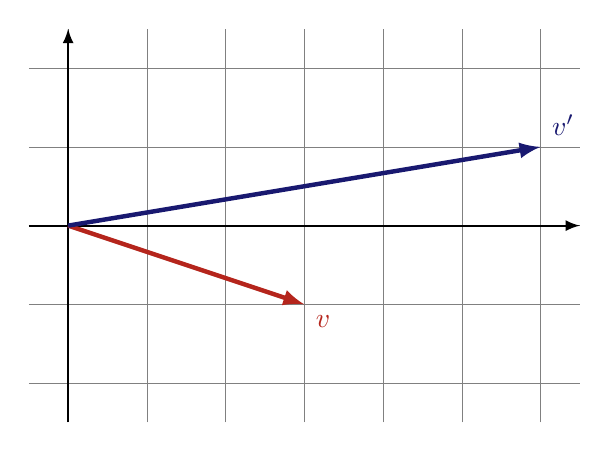
\begin{tikzpicture}
        \draw[step=1, gray,very thin] (-0.5, -2.5) grid (6.5, 2.5);
        \draw[-latex, thick] (0, -2.5) -- (0, 2.5);
        \draw[-latex, thick] (-0.5, 0) -- (6.5, 0);
        \draw[-latex, ultra thick, BrickRed] (0, 0) -- (3, -1) node[below right] {\(v\)};
        \draw[-latex, ultra thick, MidnightBlue] (0, 0) -- (6, 1) node[above right] {\(v'\)};
    \end{tikzpicture}
    \caption{Applying the linear transformation \(M\) to a vector \(v\) produces some other vector \(v'\).}
    \label{fig:Ch11-linear-trans}
\end{figure}

Sometimes, it just so happens that the resultant vector \(v'\) is a scaled version of the original vector \(v'\), i.e.
%
\begin{equation}\label{eq:Ch11-eigen-def}
    v' = Mv = \lambda v
\end{equation}
%
When this happens, the special vector \(v\) is called an \textit{eigenvector} and the corresponding scalar is called its \textit{eigenvalue}. For example, the above matrix has an eigenvector
\(
\begin{pmatrix}
    1 \\ -1
\end{pmatrix}\) because applying the matrix \(M\) to it is equivalent to scaling it by a factor of 3:
%
\[
\begin{pmatrix}
    1 & -2\\
    2 & 5
\end{pmatrix}
\begin{pmatrix}
    1 \\ -1
\end{pmatrix}
=
\begin{pmatrix}
    3 \\ -3
\end{pmatrix}
\]
%
The eigenvalue for this eigenvector is thus 3. See figure \ref{fig:Ch11-eigen}.

\begin{figure}[H]
    \centering
    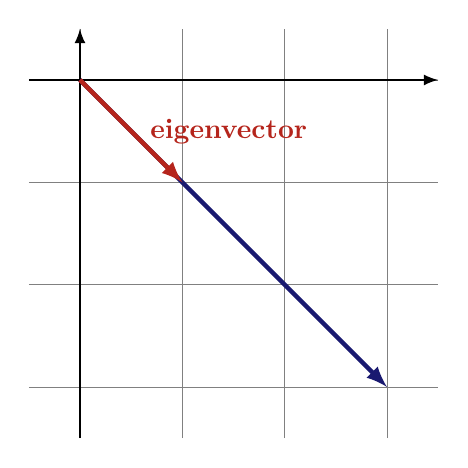
\begin{tikzpicture}[scale=1.3]
        \draw[step=1, gray,very thin] (-0.5, -3.5) grid (3.5, 0.5);
        \draw[-latex, thick] (0, -3.5) -- (0, 0.5);
        \draw[-latex, thick] (-0.5, 0) -- (3.5, 0);
        \draw[-latex, ultra thick, MidnightBlue] (0, 0) -- (3, -3);
        \draw[-latex, ultra thick, BrickRed] (0, 0) -- (1, -1) node[pos=0.5, right] {\;\textbf{eigenvector}};
    \end{tikzpicture}
    \caption{An eigenvector of \(M\) which has an eigenvalue of 3.}
    \label{fig:Ch11-eigen}
\end{figure}

Note that:
%
\begin{itemize}
    \item While the zero vector is technically a solution of \eqref{eq:Ch11-eigen-def}, this is considered a trivial solution (as it is bound to satisfy the equation for any given \(M\)) and is thus excluded from the definition of an ``eigenvector''. 
    \item A matrix can have zero, one or multiple eigenvalues.
    \item If \(v\) is an eigenvector with eigenvalue \(\lambda\), then so is \(kv\) for any nonzero scalar \(k\). This is visualised in figure \ref{fig:Ch11-eigenvalue-has-inf-eigenvectors}.
\end{itemize}

\begin{figure}[H]
    \centering
    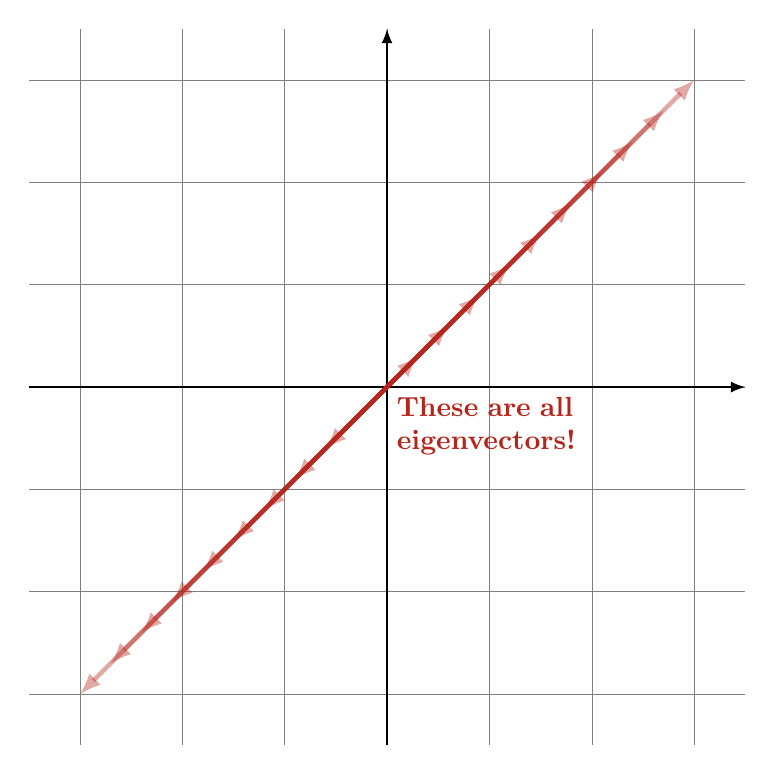
\begin{tikzpicture}[scale=1.3]
        \draw[step=1, gray,very thin] (-3.5, -3.5) grid (3.5, 3.5);
        \draw[-latex, thick] (0, -3.5) -- (0, 3.5);
        \draw[-latex, thick] (-3.5, 0) -- (3.5, 0);

        \foreach \x in {-1,-0.9, ..., -0.1, 0.1,0.2,...,1} {
            \draw[-latex, ultra thick, BrickRed, opacity=0.4] (0, 0) -- (\x*3, \x*3);
        }

        \node[below right, BrickRed, text width=3cm] at (0,0) {\textbf{These are all eigenvectors!}};
    \end{tikzpicture}
    \caption{An eigenvalue corresponds to a line of eigenvectors. (It is also possible for an eigenvalue to correspond to multiple or infinitely many lines of eigenvectors.)}
    \label{fig:Ch11-eigenvalue-has-inf-eigenvectors}
\end{figure}

Given a matrix \(M\), we can compute its eigenvector(s) \(v\) and the corresponding eigenvalue(s) \(\lambda\) by looking for solutions to the following equation.
%
\begin{equation}\label{eq:Ch11-eigen-def2}
    Mv = \lambda v
\end{equation}
%
We do this by rearranging the terms and factoring out \(v\).
%
\begin{align}
    Mv &= \lambda v \notag\\
    Mv - \lambda v &= 0 \notag\\
    Mv - (\lambda I)v &= 0 \notag\\
    (M - \lambda I) v &= 0 \notag\\
    \abs{M - \lambda I} &= 0 \tag{assuming \(v \neq 0\) by definition}
\end{align}
%
Any solution to \(\abs{M - \lambda I} = 0\) would thus give as an eigenvalue, and we can find the corresponding eigenvectors by plugging it into \eqref{eq:Ch11-eigen-def2}.

For a square matrix \(M\) of order \(n \times n\), the expression \(\abs{M - \lambda I}\) is a polynomial of order \(n\) in \(\lambda\). This is known as the \textit{characteristic polynomial} of \(M\). Each eigenvalue of \(M\) is a solution to the equation \(\abs{M - \lambda I} = 0\) (the \textit{characteristic equation}) and is thus a root of the characteristic polynomial. Since the characteristic polynomial has order \(n\), it follows from the fundamental theorem of algebra that \(M\) must have no more than \(n\) eigenvalues.





\subsubsection{Example: A matrix with no eigenvalues}

Consider the matrix
%
\(
R = 
\begin{pmatrix}
    0 & -1\\
    1 & 0
\end{pmatrix}
\).
%
This matrix rotates all vectors counterclockwise by \(90\degree\), so it is intuitively obvious that it should have no eigenvectors whatsoever. To prove this, we construct the following equation.
%
\begin{align*}
    \abs{R - \lambda I} &= 0\\
    %
    \begin{vmatrix}
        -\lambda & -1\\
        1 & -\lambda
    \end{vmatrix} &= 0\\
    %
    \lambda^2 + 1 &= 0
\end{align*}
%
This has no solution, indicating that \(R\) has no eigenvalues (or eigenvectors).




\subsubsection{Example: A matrix with one eigenvalue}

Consider the matrix
%
\(
S = 
\begin{pmatrix}
    1 & 1\\
    0 & 1
\end{pmatrix}
\).
%
(This is called a \textit{shear} mapping.) We calculate its eigenvalues as follows.
%
\begin{align*}
    \abs{S - \lambda I} &= 0\\
    %
    \begin{vmatrix}
        1-\lambda & 1\\
        0 & 1-\lambda
    \end{vmatrix} &= 0\\
    %
    (1-\lambda)^2 &= 0\\
    \lambda &= 1
\end{align*}

We then find the eigenvectors by setting \(v = \begin{pmatrix} x \\ y \end{pmatrix}\).
%
\begin{align*}
    Sv &= 1 \times v\\
    \begin{pmatrix}
        1 & 1\\
        0 & 1
    \end{pmatrix}
    \begin{pmatrix} x \\ y \end{pmatrix} &= \begin{pmatrix} x \\ y \end{pmatrix}\\
    \begin{pmatrix} x + y \\ y \end{pmatrix} &= \begin{pmatrix} x \\ y \end{pmatrix}\\
\end{align*}
%
This gives the following system of equations:
%
\[
\begin{cases}
    x + y = x\\
    y = y
\end{cases}
\]
%
which has the solution \((x, y) = (t, 0)\) for any \(t\). This means that \(S\) has the eigenvectors \(\begin{pmatrix} t \\ 0 \end{pmatrix}\) for any \(t\).



\subsubsection{Example: A matrix with multiple eigenvalues}

Suppose we want to find the eigenvectors for
%
\(
T = 
\begin{pmatrix}
    0 & -6\\
    1 & 5
\end{pmatrix}
\). We again set the following equation:
%
\begin{align*}
    \abs{T - \lambda I} &= 0\\
    \begin{vmatrix}
        -\lambda & -6\\
        1 & 5-\lambda
    \end{vmatrix} &= 0\\
    \lambda^2 - 5\lambda + 6 &= 0\\
    (\lambda - 2)(\lambda - 3) &= 0\\
    \lambda &= 2 \text{ or } 3
\end{align*}
%
We substitute each value of \(\lambda\) into the equation \(Tv = \lambda v\), with \(v\) set to \(\begin{pmatrix} x \\ y \end{pmatrix}\), in order to determine the eigenvectors.

\begin{tabular}{c|c}
    \parbox{0.5\textwidth}{
        For \(\lambda = 2\),
        \begin{align*}
            Tv &= 2v\\
            \begin{pmatrix}
                0 & -6\\
                1 & 5
            \end{pmatrix} \begin{pmatrix}
                x \\ y
            \end{pmatrix} &= \begin{pmatrix}
                2x \\ 2y
            \end{pmatrix}\\
            \begin{pmatrix}
                -6y \\ x+5y
            \end{pmatrix} &= \begin{pmatrix}
                2x \\ 2y
            \end{pmatrix}
        \end{align*}
        %
        This gives the system
        %
        \[
        \begin{cases}
            2x + 6y = 0\\
            x + 3y = 0
        \end{cases}
        \]
        %
        which has the solution
        %
        \[(x, y) = (-3t, t)\]
        %
        or
        %
        \[v = \begin{pmatrix} -3t \\ t \end{pmatrix}\]
        %
        for any \(t\).
    }
    &
    \parbox{0.5\textwidth}{
        For \(\lambda = 3\),
        \begin{align*}
            Tv &= 3v\\
            \begin{pmatrix}
                0 & -6\\
                1 & 5
            \end{pmatrix} \begin{pmatrix}
                x \\ y
            \end{pmatrix} &= \begin{pmatrix}
                3x \\ 3y
            \end{pmatrix}\\
            \begin{pmatrix}
                -6y \\ x+5y
            \end{pmatrix} &= \begin{pmatrix}
                3x \\ 3y
            \end{pmatrix}
        \end{align*}
        %
        This gives the system
        %
        \[
        \begin{cases}
            3x + 6y = 0\\
            x + 2y = 0
        \end{cases}
        \]
        %
        which has the solution
        %
        \[(x, y) = (-2t, t)\]
        %
        or
        %
        \[v = \begin{pmatrix} -2t \\ t \end{pmatrix}\]
        %
        for any \(t\).
    }
\end{tabular}



\subsubsection{The product of all eigenvalues of a matrix equals its determinant}

Here we provide a proof for the following statement:

\begin{quote}
    The determinant of the matrix \(M\) must equal the product of all \(n\) of its eigenvalues.
    %
    \begin{proof}
        Let \(M\) be a square matrix of order \(n\). We know its characteristic polynomial \(P(\lambda) = \abs{M - \lambda I}\) has order \(n\) and has \(n\) (not necessarily distinct) roots \(\lambda_1, \lambda_2, \cdots, \lambda_n\). Each of these \(n\) roots is an eigenvalue of \(M\).
        
        This allows us to express the characteristic polynomial as:
        %
        \begin{equation}\label{eq:char-poly-factored}
            P(\lambda) = k(\lambda - \lambda_1)(\lambda - \lambda_2)\cdots(\lambda - \lambda_n)
        \end{equation}
        %
        where \(k\) is a nonzero constant. By definition, we have:
        %
        \begin{align*}
            \abs{M - \lambda I} &= k(\lambda - \lambda_1)(\lambda - \lambda_2)\cdots(\lambda - \lambda_n)\\
            \begin{vmatrix}
                \boxed{\text{\textbf{?}}} - \lambda & * & \cdots & * \\
                * & \boxed{\text{\textbf{?}}} - \lambda & \cdots & * \\
                \vdots & \vdots & \ddots & \vdots \\
                * & * & \cdots & \boxed{\text{\textbf{?}}} - \lambda \\
            \end{vmatrix}
            &= k(\lambda - \lambda_1)(\lambda - \lambda_2)\cdots(\lambda - \lambda_n)\\
        \end{align*}

        Now consider the \(\lambda^n\) term on both sides.
        %
        \begin{itemize}
            \item On the left hand side, we are trying to compute the determinant of an \(n \times n\) matrix. A \(\lambda^n\) term will only be created when we multiply together the elements on the principal diagonal. Since all principal diagonal elements are of the form \(\left(\boxed{\text{\textbf{?}}} - \lambda\right)\), the determinant's \(\lambda^n\) term must equal \((-\lambda)^n\).

            \item On the right hand side, the \(\lambda^n\) term is \(k \lambda^n\).
        \end{itemize}
        %
        Combining the above gives
        %
        \begin{align*}
            (-\lambda)^n &= k \lambda^n\\
            (-1)^n &= k\\
            k &= (-1)^n
        \end{align*}
        %
        which we can substitute into \eqref{eq:char-poly-factored} to get the following relationship.
        %
        \begin{align*}
            P(\lambda) &= (-1)^n (\lambda - \lambda_1)(\lambda - \lambda_2)\cdots(\lambda - \lambda_n)\\
            \abs{M - \lambda I} &= (-1)^n (\lambda - \lambda_1)(\lambda - \lambda_2)\cdots(\lambda - \lambda_n)
        \end{align*}

        Setting \(\lambda = 0\) yields the following result.
        %
        \begin{align*}
            \abs{M} &= (-1)^n (-\lambda_1)(- \lambda_2)\cdots(- \lambda_n)\\
            &= (-1)^n \left( (-1)^n (\lambda_1 \lambda_2 \cdots \lambda_n) \right)\\
            &= (-1)^{2n} (\lambda_1 \lambda_2 \cdots \lambda_n)\\
            &= \lambda_1 \lambda_2 \cdots \lambda_n \qedhere
        \end{align*}
    \end{proof}
\end{quote}

\vspace{1em}
\hrule
\vspace{1em}


Here is an example problem that makes use of this theorem.

\vspace{1em}
\begin{mdframed}[linewidth=1pt]
\textbf{Problem}

Let \(A\) be a \(3 \times 3\) matrix, whose eigenvalues are \(\lambda_1 = 2\), \(\lambda_2 = 3\) and \(\lambda_3 = 5\).

\begin{enumerate}[label=(\alph*)]
    \item Find the eigenvalues of \(A^2\). Show that the eigenvectors of \(A^2\) are identical to those of \(A\).
    \item Given a positive integer \(n\), express the eigenvalues of \(A^n\) in terms of \(n\). Support your answer with a proof.
    \item Show that \(A\) is invertible.
    \item Find the eigenvalues of \(A^{-1}\). Show that the eigenvectors of \(A^{-1}\) are identical to those of \(A\).
    \item Consider the matrix \(B = A - 5I\). Find the eigenvalues of \(B\) and determine whether \(B\) is invertible.
\end{enumerate}
\end{mdframed}

\vspace{1em}
\begin{mdframed}[linewidth=1pt]
\textbf{Solution}

\begin{enumerate}[label=(\alph*)]
    \item As shown below, the eigenvectors of \(A^2\) are identical to those of \(A\).
    \begin{align*}
        Av &= \lambda v\\
        A^2 v &= A (\lambda v)\\
        A^2 v &= \lambda (A v) \\
        A^2 v &= \lambda (\lambda v) \\
        A^2 v &= \lambda^2 v
    \end{align*}
    %
    The last line shows that the eigenvalues of \(A^2\) are the squares of those of \(A\), i.e. 4, 9 and 25.
    
    \item The eigenvalues of \(A^n\) are \(2^n\), \(3^n\) and \(5^n\).

    \begin{proof}
        We proceed by induction. The base case is established by the fact that for \(n = 1\), the matrix \(A^n = A^1 = A\) has the eigenvalues \(\lambda = 2, 3, 5\), i.e. \(Av = \lambda v\).

        Now assume that for some positive integer \(k\), the eigenvalues of \(A^k\) are \(\lambda^k = 2^k, 3^k, 5^k\). It follows that
        %
        \begin{align*}
            A^k v &= \lambda^k v \tag{induction hypothesis}\\
            A \left(A^k v \right) &= A \left(\lambda^k v\right)\\
            A^{k+1} v &= \lambda^k (Av)\\
            A^{k+1} v &= \lambda^k (\lambda v) \tag{base case}\\
            A^{k+1} v &= \lambda^{k+1} v
        \end{align*}
        %
        which completes the induction step.
    \end{proof}

    \item \(\abs{A} = 2 \times 3 \times 5 = 30 \neq 0\), so \(A\) is invertible.
    
    \item As shown below, the eigenvectors of \(A^{-1}\) are identical to those of \(A\).
    \begin{align*}
        Av &= \lambda v\\
        A^{-1} A v &= A^{-1} (\lambda v)\\
        v &= \lambda (A^{-1} v) \\
        A^{-1} v &= \frac{1}{\lambda} v
    \end{align*}
    %
    The last line shows that the eigenvalues of \(A^{-1}\) are the reciprocals of those of \(A\), i.e. \(1/2\), \(1/3\) and \(1/5\).
    
    \item Again, the eigenvectors of \(B = A - 5I\) are identical to those of \(A\).
    %
    \begin{align*}
        Av &= \lambda v\\
        Av - 5v &= \lambda v - 5v\\
        (A-5I) v &= (\lambda - 5) v\\
        B v &= (\lambda - 5) v\\
    \end{align*}
    %
    The last line shows that the eigenvalues of \(B\) are simply \(\lambda - 5\), i.e. \(-3\), \(-2\) and \(0\). The determinant of \(B\), which is the product of the eigenvalues, is 0. This implies that \(B\) is not invertible.
\end{enumerate}
\end{mdframed}






\newpage
\section{How to count}

This section presents two counting principles which are fundamental to combinatorics.

Firstly, the \textit{multiplication principle} is used to count the number of tuples \((t_1, t_2, \cdots, t_n)\) where \(t_i\) are selected from independent sources. For any sets \(A_1, A_2, \cdots, A_n\), the cardinality of their Cartesian product is given by
%
\[
\abs{ A_1 \times A_2 \times \cdots \times A_n } = \abs{A_1} \times \abs{A_2} \times \cdots \times \abs{A_n}\text{.}
\]

Secondly, for any pair of sets \(A\) and \(B\), we have
%
\[\abs{A \cup B} = \abs{A} + \abs{B} - \abs{A \cap B}\text{.}\]
%
The same principle can be applied to calculating probabilities --- for any events \(A\) and \(B\), we have
%
\[P(A \lor B) = P(A) + P(B) - P(A \land B) \text{.}\]

\end{document}